\documentclass{ONL}

\makeatletter
\let\old@endalgorithm\endalgorithm
\renewcommand{\endalgorithm}{\old@endalgorithm\vspace*{-6mm}} % 10mm
\makeatother

\begin{document}
\abovedisplayskip=5pt\belowdisplayskip=5pt
\counterwithin{equation}{section}

\pagestyle{empty}

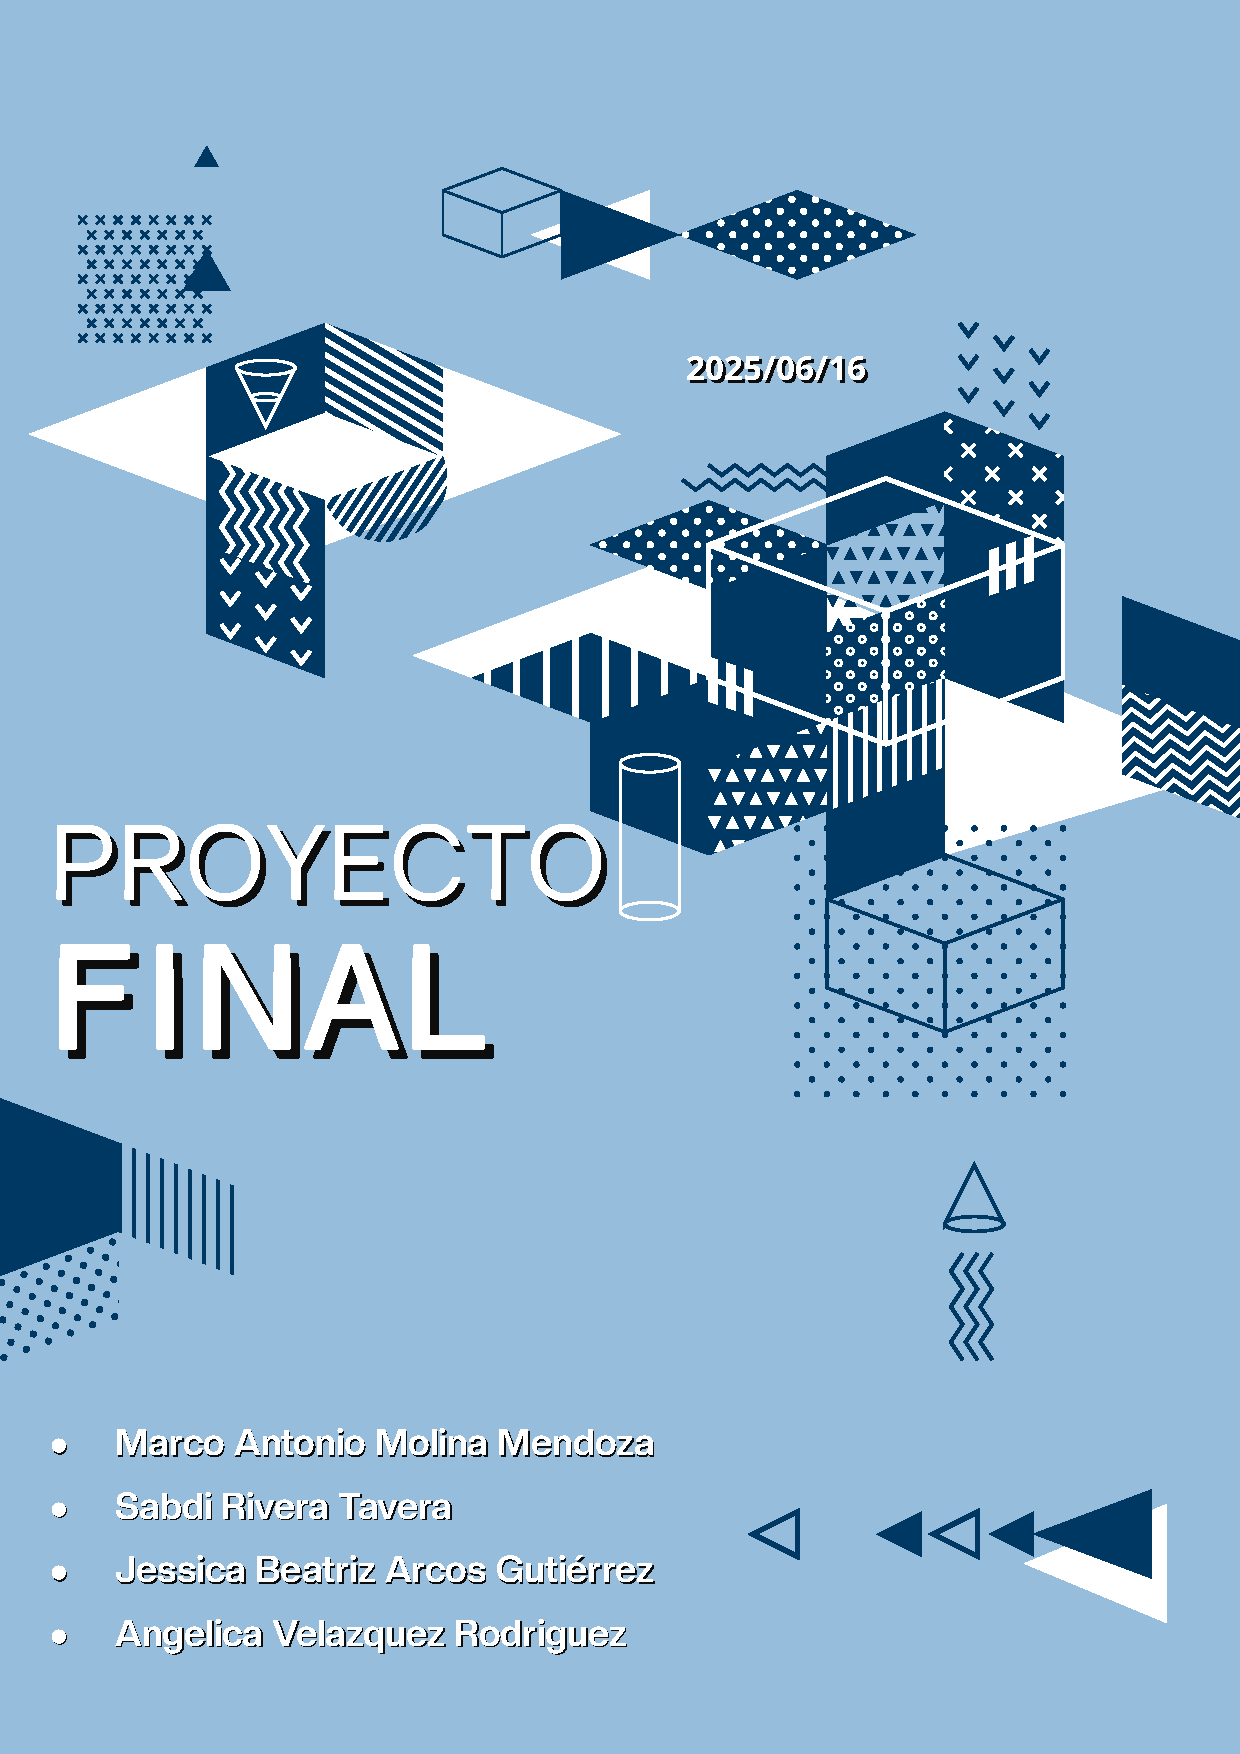
\includepdf[pages=-]{Imagenes/PortadaONL.pdf}

\newpage

%%% Tabla de contenido, lista de figuras y lista de tablas %%%
\AddToShipoutPictureBG*{\BackgroundPicCover}
\renewcommand{\contentsname}{Contenido}
\bookmarktocentry\tableofcontents\label{toc-contents}
%\listoffigures
%\listoftables
\nocite{*}

\clearpage
\pagestyle{fancy}

\chapter{Introducción}

La optimización no lineal constituye una herramienta fundamental en matemáticas aplicadas, ingeniería e inteligencia artificial, donde la búsqueda de soluciones óptimas permite resolver problemas complejos en campos como economía, diseño de sistemas y aprendizaje automático. Sin embargo, la diversidad de problemas de optimización (desde funciones suaves hasta paisajes multimodales con múltiples óptimos locales) plantea un desafío crítico: \emph{no existe un algoritmo universalmente superior}. La elección del método depende de factores como la naturaleza de la función objetivo, el costo computacional, la disponibilidad de derivadas y la precisión requerida.

\section*{Motivación}

Este proyecto surge de la necesidad de evaluar científicamente el rendimiento de métodos de optimización en escenarios realistas. Muchos estudios comparativos se limitan a pruebas con puntos iniciales únicos, lo que puede sesgar los resultados. Aquí, implementamos una metodología rigurosa mediante \textbf{técnicas de multistart} con 2,500 puntos iniciales distribuidos uniformemente, garantizando robustez estadística y reproducibilidad. Además, seleccionamos siete funciones de prueba (seis multimodales y una cuadrática) que representan desafíos típicos en aplicaciones científicas y técnicas, desde la clásica Booth hasta la compleja Goldstein-Price.

\section*{Contribución}

Este trabajo no solo valida teóricamente los métodos estudiados, sino que ofrece un \emph{análisis práctico} mediante implementaciones en MATLAB, código reproducible y resultados detallados para cada función. Los hallazgos destacan \emph{trade-offs} entre velocidad, precisión y requerimientos computacionales, demostrando, por ejemplo, la eficiencia de Newton en funciones cuadráticas frente a la resiliencia de Hooke-Jeeves en problemas sin derivadas. Esta comparación sistemática sirve como referencia para investigadores e ingenieros que enfrentan problemas de optimización en entornos multidisciplinarios.

\chapter{Marco teórico}

\section{Método de descenso con máxima pendiente}

El método de descenso con máxima pendiente, también conocido como método de Cauchy o steepest descent, es un algoritmo iterativo ampliamente utilizado en optimización no lineal. Su objetivo es encontrar el mínimo local de una función diferenciable en $\mathbb{R}^n$.

En cada iteración, el método de descenso requiere calcular una dirección de búsqueda $v$ y un tamaño de paso $\alpha$, actualizando el punto actual $x^{(k)}$ a un nuevo punto $x^{(k + 1)}$ mediante la fórmula
$$x^{(k + 1)} = x^{(k)} + \alpha v.$$
La dirección de descenso se elige como el negativo del gradiente, $-\nabla f\left(x^{(k)}\right)$, ya que esta es la dirección de máximo decremento de la función. El tamaño de paso $\alpha_k$ se determina resolviendo un problema de minimización unidimensional a lo largo de la dirección de descenso, es decir,
$$\alpha_k = \arg \min_{\alpha \geq 0} \left\{f\left(x^{(k)} + \alpha_k v_k\right)\right\}.$$
Este proceso se repite hasta que se alcanza un punto óptimo local.

\subsection{Condiciones de Wolfe}

Las Condiciones de Wolfe son un conjunto de criterios para asegurar que el tamaño de paso en cada iteración conduzca a una reducción suficiente de la función objetivo y a un progreso adecuado hacia el mínimo. Las Condiciones de Wolfe constan de dos partes:
\begin{itemize}
    \item Condición de Armijo: Esta condición dada por $f\left(x^{(k)} + \alpha_k v_k\right) \leq f\left(x^{(k)}\right) + c_1 \alpha_k \nabla f\left(x^{(k)}\right)^{\top} v_k$, donde $0 \leq c_1 \leq 1$, asegura que la disminución en la función objetivo sea proporcional al tamaño del paso y la derivada direccional.
    \item Condición de curvatura: Esta condición dada por $\nabla f\left(x^{(k)} + \alpha_k v_k\right)^{\top} v_k \geq c_2 \nabla f\left(x^{(k)}\right)^{\top} v_k$, donde $c_1 \leq c_2 \leq 1$, asegura que el tamaño del paso no sea demasiado pequeño. 
\end{itemize}

\newpage

\section{Método de Newton para varias variables}

El método de Newton se basa en aproximar la función objetivo mediante una expansión cuadrática de Taylor alrededor del punto actual $x^{(k)}$. Esta aproximación tiene en cuenta tanto el gradiente $\nabla f\left(x^{(k)}\right)$ como la matriz Hessiana $H\left(x^{(k)}\right)$. El objetivo es minimizar la siguiente función,
$$q(x) = f\left(x^{(k)}\right) + \left(x - x^{(k)}\right)^{\top} g^{(k)} + \frac{1}{2} \left(x - x^{(k)}\right)^{\top} H\left(x^{(k)}\right) \left(x - x^{(k)}\right)$$
donde $g^{(k)} = \nabla f\left(x^{(k)}\right)$ y $H := \nabla^2 f\left(x^{(k)}\right)$, que es una aproximación cuadrática a la función original. El mínimo de dicha función se encuentra cuando
$$H\left(x^{(k)}\right)^{-1} g^{(k)} + \left(x - x^{(k)}\right) = 0.$$
De esta manera, la nueva iteración se calcula como
$$x^{(k + 1)} = x^{(k)} - H\left(x^{(k)}\right)^{-1} g^{(k)}.$$
Si la matriz Hessiana es definida positiva en el punto $x^{(k)}$, entonces $H\left(x^{(k)}\right)^{-1} g^{(k)}$ nos llevará a un mínimo local de la función. El método de Newton no siempre garantiza el descenso; es decir, no siempre se cumple que $f\left(x^{(k + 1)}\right) < f\left(x^{(k)}\right)$. Además, calcular la Hessiana y resolver el sistema lineal en cada iteración puede ser computacionalmente costoso, especialmente para problemas de gran escala. La Hessiana también puede ser singular, lo que impide la inversión.

\subsection{Modificación Levenberg-Marquardt}

Para mitigar algunos de los problemas del método de Newton, como la falta de definitud positiva de la matriz Hessiana, se introduce una modificación llamada modificación de Levenberg-Marquardt. Esta técnica ajusta la matriz Hessiana de la siguiente manera
$$x^{(k + 1)} = x^{(k)} - \left[H\left(x^{(k)}\right) + \mu_k I\right]^{-1} g^{(k)},$$
donde $\mu_k$ es un parámetro que se ajusta durante el proceso. Si $\mu_k$ es grande, el comportamiento del método se asemeja al del método de máxima pendiente con un paso pequeño, mientras que si $\mu_k$ es pequeño, el algoritmo se aproxima al método de Newton.

\section{Método de Cuasi-Newton}

El Método Cuasi-Newton es una modificación del método de Newton que busca aproximar la inversa de la matriz Hessiana de la función objetivo de forma iterativa. Esto se hace para reducir el costo computacional de calcular la Hessiana en cada iteración, como lo requiere el método de Newton, y para evitar problemas cuando la Hessiana es singular o no definida positiva. En cada iteración, se añade una matriz de corrección $U_k$ a la matriz $H_k$ para obtener la siguiente aproximación:
$$H_{k+1} = H_k + U_k.$$
\newpage\noindent
Esta actualización se realiza para incorporar información sobre la curvatura de la función objetivo, basándose en los cambios observados en los gradientes. La condición de Cuasi-Newton, derivada de la expansión de Taylor de segundo orden, establece que
$$g_{k+1} - g_k \approx H(x_k) d_k$$
donde $g_{k + 1} := \nabla f(x_k + d_k)$ y $d_k = x_{k+1} - x_k$ es el paso dado en la iteración.

\subsection{Rango uno}

El método de rango uno es un método Cuasi-Newton específico que calcula la actualización de la inversa de la Hessiana mediante la siguiente fórmula:
$$H_{k+1} = H_k + \frac{\left(\Delta x^{(k)} - H_k \Delta g^{(k)}\right) \left(\Delta x^{(k)} - H_k \Delta g^{(k)}\right)^{\top}}{\Delta\left. g^{(k)} \right.^{\top} \left(\Delta x^{(k)} - H_k \Delta g^{(k)}\right)}$$
para obtener $d^{(k)} = -H_k g^{(k)}$ donde
$$x^{(k+1)} = x^{(k)} + \alpha_k d^{(k)}$$
y $\alpha_k$ es el tamaño de paso.

\subsection{Rango dos}
El método de rango dos (DFP) es un método Cuasi-Newton que actualiza la aproximación de la inversa de la Hessiana garantizando que si $H_k$ es definida positiva, entonces $H_{k+1}$ también lo será. La fórmula de actualización es:

\[
H_{k+1} = H_k + \frac{\Delta x^{(k)}\Delta x^{(k)\top}}{\Delta x^{(k)\top}\Delta g^{(k)}} - \frac{H_k \Delta g^{(k)} \Delta g^{(k)\top} H_k}{\Delta g^{(k)\top} H_k \Delta g^{(k)}}
\]

donde: $\Delta x^{(k)} = x^{(k+1)} - x^{(k)}$ (cambio en el punto), $\Delta g^{(k)} = \nabla f(x^{(k+1)}) - \nabla f(x^{(k)})$ (cambio en el gradiente),$H_k$ es la aproximación actual de la inversa de la Hessiana.

\section{Método de gradientes conjugados}

El método de Gradientes Conjugados es un algoritmo iterativo para resolver sistemas de ecuaciones lineales y optimización no lineal. Es particularmente eficiente para minimizar funciones cuadráticas y puede extenderse a funciones no cuadráticas. 

\subsection[Fórmulas para \texorpdfstring{$\beta_k$}{bk}]{Fórmulas para \texorpdfstring{\boldmath$\beta_k$}{bk}}

\begin{itemize}
    \item Hestenes-Stiefel: $\beta_k^{HS} = \dfrac{\nabla f(x^{k+1})^T (\nabla f(x^{k+1}) - \nabla f(x^k))}{d^{kT}(\nabla f(x^{k+1}) - \nabla f(x^k))}$.
    \item Polak-Ribière: $\beta_k^{PR} = \dfrac{\nabla f(x^{k+1})^T (\nabla f(x^{k+1}) - \nabla f(x^k))}{\nabla f(x^k)^T \nabla f(x^k)}$.
    \item Fletcher-Reeves: $\beta_k^{FR} = \dfrac{\nabla f(x^{k+1})^T \nabla f(x^{k+1})}{\nabla f(x^k)^T \nabla f(x^k)}$.
\end{itemize}


\chapter{Metodología}

La metodología de este proyecto se centra en la evaluación de diferentes métodos de optimización no lineal sin restricciones. Para ello, se busca el punto óptimo de diversas funciones objetivo utilizando cinco métodos distintos: Descenso con Máxima Pendiente, Método de Newton, Método Cuasi-Newton, Gradientes Conjugados y el algoritmo de Hooke-Jeeves.

Para garantizar la robustez y fiabilidad de los resultados, se implementará la técnica de \emph{multistart}. En lugar de evaluar cada método desde un único punto inicial, se generan $N$\footnote{Como en nuestras anteriores tareas, asignaremos 2500 al valor de $N$.} puntos iniciales aleatorios uniformemente distribuidos dentro del dominio definido para cada función. Esto permite mitigar el riesgo de obtener resultados sesgados por la elección de un único punto de partida, que podría tener ventajas específicas o conducir a óptimos locales. Para asegurar la reproducibilidad de los experimentos, se controla el generador de números aleatorios estableciendo una semilla fija en el código, de modo que cada conjunto de puntos iniciales se utilice de manera consistente para cada método y función.

Una vez generados los $N$ puntos iniciales, cada uno de los cinco métodos de optimización se ejecuta para cada punto. De cada ejecución, se recopilan los siguientes resultados:
\begin{itemize}
    \item Número de iteraciones: Este indicador refleja el costo computacional del método en términos de evaluaciones de la función objetivo.
    \item Punto óptimo encontrado: Este valor es crucial para verificar la correcta convergencia del método y para identificar si algún punto inicial no converge a la solución esperada.
    \item Función evaluada en el punto óptimo: Este valor es el resultado de sustituir el punto óptimo encontrado en la función objetivo, lo que indica el valor mínimo (o máximo) alcanzado por la función.
    \item Error: Este parámetro mide la norma de la diferencia entre el punto óptimo encontrado por el método y el verdadero punto óptimo de la función, lo que permite evaluar la precisión del algoritmo.
\end{itemize}
Finalmente, se realizará un análisis comparativo de los resultados obtenidos para cada método. Este análisis permitirá evaluar la efectividad, eficiencia y fiabilidad de cada algoritmo en la resolución de problemas de optimización.

\newpage

\section{Programas de \textsc{Matlab}}

\subsection{Algoritmo de Máxima Pendiente}
\begin{matlab}
    unction [best_x, best_val, tiempo_ejecucion, num_evaluaciones, x_inicios, resultados] = multistart_maxima_pen_interv(f, grad_f, num_inicios, lb, ub)
    % Multistart con descenso por máxima pendiente y registro de puntos iniciales
    % Con error y número de iteraciones
    % lb: límite inferior 
    % ub: límite superior 
    
    tic; 
    num_evaluaciones = 0;
    best_val = Inf;
    best_x = [];
    x_inicios = zeros(2, num_inicios); 
    resultados = struct('x0', {}, 'x_opt', {}, 'f_val', {}, 'evals', {}, 'iterations', {}, 'error', {});

    rng(42); % Fija semilla aleatoria para reproducibilidad

    for i = 1:num_inicios
     
        x0 = lb + (ub - lb) .* rand(2,1);
        x_inicios(:, i) = x0;

        % Optimización desde x0
        [x_opt, evals, iterations, err] = maxima_pen_interv(f, grad_f, x0);
        val = f(x_opt);
        num_evaluaciones = num_evaluaciones + evals + 1; % +1 por evaluación final

        % Guarda resultados individuales
        resultados(i).x0 = x0;
        resultados(i).x_opt = x_opt;
        resultados(i).f_val = val;
        resultados(i).evals = evals;
        resultados(i).iterations = iterations;
        resultados(i).error = err;

        % Actualiza mejor solución global
        if val < best_val
            best_val = val;
            best_x = x_opt;
        end
    end
    tiempo_ejecucion = toc; 
end

% -----------------------------------------------------------------------
function [x_opt, num_evaluaciones, iterations, error] = maxima_pen_interv(f, grad_f, x0)
    % Descenso por gradiente con búsqueda lineal exacta
    % Número de iteraciones y error final
    
    tol = 1e-6;
    max_iter = 1000;
    iterations = 0;
    xk = x0(:);
    num_evaluaciones = 0;
    error = Inf;

    while norm(grad_f(xk)) > tol && iterations < max_iter
        vk = -grad_f(xk); % Dirección de descenso
        % Búsqueda lineal (fminbnd usa ~30 evaluaciones internas)
        alpha_k = fminbnd(@(alpha) f(xk + alpha * vk), 0, 1);
        xk = xk + alpha_k * vk;
        iterations = iterations + 1;
        num_evaluaciones = num_evaluaciones + 30; % Estimación conservadora
        error = norm(grad_f(xk));
    end
    x_opt = xk;
end

% -------------------------------------------------------------------------
% Función 
f1 = @(x) x(1)^2 + 2*x(2)^2 - 0.3*cos(3*pi*x(1)) - 0.4*cos(4*pi*x(2)) + 0.7;
% Gradiente numérico 
grad_f1 = @(x) [
    (f1(x + [1e-6; 0]) - f1(x - [1e-6; 0])) / (2e-6);
    (f1(x + [0; 1e-6]) - f1(x - [0; 1e-6])) / (2e-6)
];

% -------------------------------------------------------------------------

num_reinicios = 30;
lb = [-100; -100]; % Límites inferiores 
ub = [100; 100];   % Límites superiores 
[best_x, best_val, tiempo, evals, x_inicios, resultados] = multistart_maxima_pen_interv(f1, grad_f1, num_reinicios, lb, ub);

% Mostrar resultados en consola
disp('=== RESULTADOS ===');
disp(['Mejor mínimo encontrado: [', num2str(best_x'), ']']);
disp(['Valor de la función: ', num2str(best_val)]);
disp(['Tiempo total: ', num2str(tiempo), ' segundos']);
disp(['Evaluaciones de f(x): ', num2str(evals)]);

% Mostrar estadísticas de iteraciones y errores
iterations_array = [resultados.iterations];
error_array = [resultados.error];
disp(['Iteraciones promedio por ejecución: ', num2str(mean(iterations_array))]);
disp(['Error promedio final: ', num2str(mean(error_array))]);
disp(['Máximo error final: ', num2str(max(error_array))]);
\end{matlab}
\subsection{Algoritmo del Método de Newton}
\begin{matlab}
    function newton_multivariable_multistart_2500_symbolic()
    % Limpiar entorno
    clear; clc;

    % Definir variables simbólicas
    syms x1 x2
    vars = [x1; x2];

    % Definir la función simbólica (Goldstein-Price simplificada)
 f_expr = (1.5 - x1 + x1*x2)^2 + (2.25 - x1 + x1*x2^2)^2 + (2.625 - x1 + x1*x2^3)^2;
    % Calcular gradiddente y Hessiana simbólicas
    grad_f_sym = gradient(f_expr, vars);
    H_f_sym = hessian(f_expr, vars);

    % Convertir a funciones numéricas
    f = matlabFunction(f_expr, 'Vars', {vars});
    grad_f = matlabFunction(grad_f_sym, 'Vars', {vars});
    H_f = matlabFunction(H_f_sym, 'Vars', {vars});

    % Parámetros
    max_iter = 100;
    tol = 1e-6;
    num_starts = 2500;
    rango = [-5, 5];

    % Inicialización del mejor resultado
    mejor_valor = inf;
    mejor_resultado = struct();

    for intento = 1:num_starts
        x0 = rango(1) + (rango(2) - rango(1)) * rand(2,1);
        x = x0;
        x_prev = inf(size(x0));
        iter = 0;
        converged = false;
        llamadas_funcion = 0;

        while iter < max_iter && ~converged
            g = grad_f(x); g = g(:);  % vector columna
            H_current = H_f(x);

            if iter > 0
                error = norm(x - x_prev);
            else
                error = inf;
            end

            if iter > 0 && error < tol
                converged = true;
                break;
            end

            % Comprobar condición numérica Hessiana
            if rcond(H_current) < 1e-12
                break;
            end

            x_prev = x;
            d = -H_current \ g;
            x = x + d;

            iter = iter + 1;
            llamadas_funcion = llamadas_funcion + 1;
        end

        valor_final = f(x);
        llamadas_funcion = llamadas_funcion + 1;
        grad_final = grad_f(x); grad_final = grad_final(:);

        if valor_final < mejor_valor
            mejor_valor = valor_final;
            mejor_resultado.x0 = x0;
            mejor_resultado.x_opt = x;
            mejor_resultado.valor_funcion = valor_final;
            mejor_resultado.gradiente = grad_final;
            mejor_resultado.error = norm(x - x_prev);
            mejor_resultado.iteraciones = iter;
            mejor_resultado.llamadas_funcion = llamadas_funcion;
        end
    end

    % Mostrar solo el mejor resultado
    fprintf('Mejor resultado encontrado (entre %d puntos):\n', num_starts);
    fprintf('Punto inicial:      [%.6f, %.6f]\n', mejor_resultado.x0(1), mejor_resultado.x0(2));
    fprintf('Punto óptimo:       [%.6f, %.6f]\n', mejor_resultado.x_opt(1), mejor_resultado.x_opt(2));
    fprintf('Valor función:      %.6f\n', mejor_resultado.valor_funcion);
    fprintf('Gradiente óptimo:   [%.6f, %.6f]\n', mejor_resultado.gradiente(1), mejor_resultado.gradiente(2));
    fprintf('Error final:        %.6f\n', mejor_resultado.error);
    fprintf('Iteraciones:        %d\n', mejor_resultado.iteraciones);
    fprintf('Llamadas función:   %d\n', mejor_resultado.llamadas_funcion);
end
\end{matlab}
\subsection{Algoritmo de Cuasi-Newton Rango 1}

\begin{matlab}
% Parámetros comunes
a = -10; b = 10;            % Límites del dominio
n_points = 2500;            % Número de puntos iniciales
dim = 2;                    % Dimensión del problema
true_opt = [1, 3];          % Óptimo verdadero
max_iter = 1000;            % Máximo de iteraciones por ejecución
tol = 1e-6;                 % Tolerancia de convergencia

% Generar 2500 puntos iniciales uniformemente distribuidos
rng(1); % Fijar semilla para reproducibilidad
initial_points = a + (b-a)*rand(n_points, dim);

% Definir la función objetivo
objective_func = @(x) (x(1) + 2*x(2) - 7)^2 + (2*x(1) + x(2) - 5)^2; % Función de la sección 4.2

% Llamar al optimizador
[opt_x, fval, best_iter, err] = quasi_newton_rango1_ms(...
    objective_func, initial_points, a, b, true_opt, max_iter, tol);

% Mostrar resultados
fprintf('Cuasi-Newton Rango 1:\n');
fprintf('  Punto óptimo: [%.6f, %.6f]\n', opt_x(1), opt_x(2));
fprintf('  Valor función: %.6f\n', fval);
fprintf('  Iteraciones: %d\n', best_iter);
fprintf('  Error: %.6f\n', err);

% FUNCIÓN PRINCIPAL: Cuasi-Newton Rango 1 con MultiStart
function [best_x, best_fval, best_iter, best_err] = quasi_newton_rango1_ms(...
    f, initial_points, a, b, true_opt, max_iter, tol)
    
    n_points = size(initial_points, 1);
    dim = size(initial_points, 2);
    
    best_fval = inf;
    best_x = [];
    best_iter = 0;  % Almacena iteraciones de la mejor ejecución
    
    for i = 1:n_points
        x0 = initial_points(i,:);
        [x_opt, fval, iter, success] = quasi_newton_rango1(...
            f, x0, dim, a, b, max_iter, tol);
        
        % Guardar iteraciones SOLO si es la mejor ejecución
        if success && fval < best_fval
            best_fval = fval;
            best_x = x_opt;
            best_iter = iter;  % Guarda iteraciones de esta ejecución
        end
    end
    
    best_err = norm(best_x - true_opt);
end

% ALGORITMO DE CUASI-NEWTON RANGO 1
function [x_opt, fval, iter, success] = quasi_newton_rango1(...
    f, x0, dim, a, b, max_iter, tol)
    
    % Inicialización
    x = x0(:); % Convertir a vector columna
    H = eye(dim); % Matriz inicial identidad
    iter = 0;
    success = false;
    n_restart = 0; % Contador para reinicio
    
    % Almacenar puntos para evitar ciclos infinitos
    x_history = zeros(dim, max_iter+1);
    x_history(:,1) = x;
    
    while iter < max_iter
        iter = iter + 1;
        
        % Calcular gradiente con diferencias finitas
        g = gradiente(f, x);
        
        % Verificar convergencia
        if norm(g) < tol
            success = true;
            break;
        end
        
        % Reiniciar cada n iteraciones (n = dimensión)
        if n_restart >= dim
            d = -g; % Dirección de descenso más pronunciado
            H = eye(dim); % Reiniciar matriz H
            n_restart = 0; % Reiniciar contador
        else
            % Calcular dirección de búsqueda
            d = -H * g;
            n_restart = n_restart + 1;
        end
        
        % Verificar dirección de descenso
        if g' * d >= 0
            d = -g; % Usar descenso más pronunciado
            H = eye(dim); % Reiniciar matriz H
            n_restart = 0;
        end
        
        % Búsqueda lineal exacta (sección dorada)
        alpha = golden_section_search(f, x, d, a, b, 100);
        
        % Actualizar punto
        x_new = x + alpha * d;
        
        % Asegurar que está dentro de los límites
        x_new = max(min(x_new, b), a);
        
        % Calcular nuevo gradiente
        g_new = gradiente(f, x_new);
        
        % Calcular diferencias
        delta_x = x_new - x;
        delta_g = g_new - g;
        
        % Verificar condición de actualización
        denom = delta_g' * (delta_x - H * delta_g);
        
        % Actualizar matriz H si se cumple la condición
        if abs(denom) > 1e-10
            u = delta_x - H * delta_g;
            H = H + (u * u') / denom;
        end
        
        % Verificar si la matriz H es definida positiva
        if ~isdefinite(H)
            % Si no es DP, usar descenso más pronunciado en la próxima iteración
            n_restart = dim; % Forzar reinicio
        end
        
        % Actualizar para siguiente iteración
        x = x_new;
        x_history(:,iter+1) = x;
        
        % Verificar convergencia en posición
        if norm(delta_x) < tol
            success = true;
            break;
        end
        
        % Detectar estancamiento
        if iter > 10 && norm(x - x_history(:,iter-5)) < tol
            success = true;
            break;
        end
    end
    
    x_opt = x';
    fval = f(x_opt);
end


% FUNCIÓN PARA CALCULAR EL GRADIENTE (DIFERENCIAS FINITAS)
function g = gradiente(f, x)
    h = 1e-8; % Tamaño del paso
    n = length(x);
    g = zeros(n, 1);
    
    for i = 1:n
        e_i = zeros(n, 1);
        e_i(i) = 1;
        
        f_forward = f(x + h*e_i);
        f_backward = f(x - h*e_i);
        
        g(i) = (f_forward - f_backward) / (2*h);
    end
end

% BÚSQUEDA LINEAL CON MÉTODO DE LA SECCIÓN DORADA
function alpha = golden_section_search(f, x, d, a, b, max_iter)
    % Parámetros de la sección dorada
    golden_ratio = (sqrt(5)-1)/2;
    tol = 1e-6;
    
    % Establecer intervalo inicial
    low = 0;
    high = 1;
    
    % Expandir intervalo si es necesario
    while f(x + high*d) < f(x + low*d)
        high = 2*high;
    end
    
    % Puntos iniciales
    x1 = high - golden_ratio*(high - low);
    x2 = low + golden_ratio*(high - low);
    
    f1 = f(x + x1*d);
    f2 = f(x + x2*d);
    
    % Iteraciones de la sección dorada
    for i = 1:max_iter
        if (high - low) < tol
            break;
        end
        
        if f1 < f2
            high = x2;
            x2 = x1;
            f2 = f1;
            x1 = high - golden_ratio*(high - low);
            f1 = f(x + x1*d);
        else
            low = x1;
            x1 = x2;
            f1 = f2;
            x2 = low + golden_ratio*(high - low);
            f2 = f(x + x2*d);
        end
    end
    
    alpha = (low + high)/2;
end

% VERIFICAR SI UNA MATRIZ ES DEFINIDA POSITIVA
function result = isdefinite(A)
    % Se intenta realizar la descomposición de Cholesky
    [~, p] = chol(A);
    result = (p == 0);
end
\end{matlab}

\subsection{Algoritmo del Método de Gradientes Conjugados}
\begin{matlab}
clc; clear;

fprintf('=== MultiInicio manual con gradientes conjugados ===\n');

% Variables simbólicas para la función y el gradiente
syms x y

%===============FUNCIONES A EVALUAR=================
% 1) 17. Función Bohachevsky: x(1)^2 + 2*x(2)^2 - 0.3*cos(3*pi*x(1)) - 0.4*cos(4*pi*x(2)) + 0.7;
% 2) 24. Función Booth: (x(1) + 2*x(2) - 7)^2 + (2*x(1) + x(2) - 5)^2;
% 3) 40. Goldstein-Price: (1 + (x(1) + x(2) + 1)^2 * (19 - 14*x(1) + 3*x(1)^2 - 14*x(2) + 6*x(1)*x(2) + 3*x(2)^2)) * ...
%     (30 + (2*x(1) - 3*x(2))^2 * (18 - 32*x(1) + 12*x(1)^2 + 48*x(2) - 36*x(1)*x(2) + 27*x(2)^2));
% 4) 25. Función Matyas: 0.26*(x(1)^2 + x(2)^2) - 0.48*x(1)*x(2);
% 5) 29. Función Three Hump Camel: 2*x(1)^2 - 1.05*x(1)^4 + (x(1)^6)/6 + x(1)*x(2) + x(2)^2;
% 6) 34. Función Eason: -cos(x(1))*cos(x(2))*exp(-(x(1)-pi)^2 - (x(2)-pi)^2);
% 7) 36. Función Beale:  @(x) (1.5 - x(1) + x(1)*x(2))^2 + (2.25 - x(1) + x(1)*x(2)^2)^2 + (2.625 - x(1) + x(1)*x(2)^3)^2;


funcion = @(x) x(1)^2 + 2*x(2)^2 - 0.3*cos(3*pi*x(1)) - 0.4*cos(4*pi*x(2)) + 0.7;
gradiente = @(x) [
    2*x(1) + 0.9*pi*sin(3*pi*x(1));
    4*x(2) + 1.6*pi*sin(4*pi*x(2))
];

% Parámetros de MultiInicio
num_intentos = 2500;
lim_inf = [-100; -100];
lim_sup = [100; 100];

% Inicializar valores
% Inicializar valores
mejor_error = inf;  % Ahora el criterio será el error

for i = 1:num_intentos
    x_inicial = lim_inf + (lim_sup - lim_inf) .* rand(2,1);

    % Llamar al método del gradiente conjugado
    [x_optimo, gradiente_optimo, valor_funcion, iteraciones, llamadas_f] = gradiente_conjugado(x_inicial, funcion, gradiente);

    % Calcular el error actual
    error_actual = norm(x_optimo - x_inicial);

    % Comparar con el mejor error hasta ahora
    if error_actual < mejor_error
        mejor_error = error_actual;
        mejor_valor = valor_funcion;
        mejor_x0 = x_inicial;
        mejor_xopt = x_optimo;
        mejor_grad = gradiente_optimo;
        mejor_iters = iteraciones;
        mejor_llamadas = llamadas_f;
    end
end



% Mostrar solo la mejor ejecución
fprintf('\n=== Mejor ejecución de %d intentos ===\n', num_intentos);
fprintf('Punto inicial: (%.6f, %.6f)\n', mejor_x0(1), mejor_x0(2));
fprintf('Punto óptimo:  (%.6f, %.6f)\n', mejor_xopt(1), mejor_xopt(2));
fprintf('Valor de la función: %.10f\n', mejor_valor);
fprintf('Gradiente en óptimo: (%.10f, %.10f)\n', mejor_grad(1), mejor_grad(2));
fprintf('Error ||x_opt - x0||: %.10f\n', mejor_error);
fprintf('Iteraciones:   %d\n', mejor_iters);
fprintf('Llamadas a f:  %d\n', mejor_llamadas);

%% Función: gradiente conjugado
function [x_optimo, gradiente_optimo, valor_funcion, iteraciones, llamadas_f] = gradiente_conjugado(x0, funcion, gradiente)
    x_k = x0(:);
    g_k = gradiente(x_k);
    d_k = -g_k;
    tolerancia = 1e-9;
    iter_max = 3000;
    iteraciones = 0;
    llamadas_f = 0;

    while iteraciones < iter_max
        phi = @(alfa) funcion(x_k + alfa*d_k);
        alfa_k = fminbnd(phi, 0, 1);
        llamadas_f = llamadas_f + 1;

        x_k1 = x_k + alfa_k*d_k;
        g_k1 = gradiente(x_k1);
        llamadas_f = llamadas_f + 1;

        if norm(g_k1) < tolerancia
            break;
        end

        if mod(iteraciones, length(x_k)) == 0
            d_k1 = -g_k1;
        else
            beta_k = (g_k1'*g_k1) / (g_k'*g_k);
            d_k1 = -g_k1 + beta_k * d_k;
        end

        x_k = x_k1;
        g_k = g_k1;
        d_k = d_k1;
        iteraciones = iteraciones + 1;
    end

    x_optimo = x_k1;
    gradiente_optimo = g_k1;
    valor_funcion = funcion(x_optimo);
    llamadas_f = llamadas_f + 1;
end
\end{matlab}


\chapter{Funciones a optimizar}

En este capítulo se presenta el núcleo experimental del proyecto: el análisis comparativo de cinco métodos de optimización aplicados a siete funciones de prueba. Se ha elegido un conjunto variado de funciones de prueba, considerando aspectos como la complejidad de su superficie, la presencia de múltiples óptimos locales, la dimensión del problema y la sensibilidad a las condiciones iniciales. Cada función ha sido seleccionada con el objetivo de cubrir un amplio espectro de escenarios que suelen encontrarse en problemas de optimización del mundo real.

\section{Función de Bohachevsky} % 17

La función de Bohachevsky está definida como:
$$f_1(\mathbf{x}) = x_1^2 + 2x_2^2 - 0.3 \cos(3\pi x_1) - 0.4\cos(4\pi x_2) + 0.7.$$
Está función la evaluaremos en $x_i \in [-100, 100]$, para $i = 1, 2$. En \citep{sfuoptimization}, se menciona que el mínimo global está en $\mathbf{x}^* = (0, 0)$ y al evaluarlo en la función se obtiene $f_1\left(\mathbf{x}^*\right) = 0$.
\begin{figure}[H]
    \centering
    \subfloat[Gráfica de la función de Bohachevsky]{
    \begin{tikzpicture}
        \begin{axis}[
            xlabel=$x_1$,
            ylabel=$x_2$,
            xtick distance=50,
            ytick distance=50,
            ztick distance=10000,
            grid=major,
            domain=-100:115,
            y domain=-115:110,
            view={60}{30},
            width=0.49\textwidth,
        ]
            \addplot3[surf, samples=30] {x^2 + 2*y^2 - 0.3*cos(deg(3*pi*x)) - 0.4*cos(deg(4*pi*y)) + 0.7};
        \end{axis}
    \end{tikzpicture}
    }
    \subfloat[Curvas de nivel de la función de Bohachevsky]{
    \begin{tikzpicture}
        \begin{axis}[
            xlabel=$x_1$,
            ylabel=$x_2$,
            domain=-100:100,
            y domain=-100:100,
            view={0}{90},
            width=0.49\textwidth,
        ]
        \addplot3[contour gnuplot={
            levels={0, 500, 1000, 2000, 4000, 8000, 12000, 16000, 20000, 24000, 28000, 30000},
            labels=false,},
            thick,
            samples=30] gnuplot {x**2 + 2*y**2 - 0.3*cos(3*pi*x) - 0.4*cos(4*pi*y) + 0.7};
        \end{axis}
    \end{tikzpicture}
    }
    \caption{}
\end{figure}

\newpage\noindent
Al correr nuestros programas, obtenemos la siguiente tabla:
\begin{table}[H]
    \begin{NiceTabular}{ccccc}[hvlines-except-borders,cell-space-limits=5pt,rules={color=white,width=1pt}]
        \CodeBefore
        \rowcolor{cw0!80}{1}
        \rowcolors{2}{cw2!70!white}{cw1!30!white}
        \Body
        \RowStyle[color=white]{}
        \RowStyle{\bfseries}
        Método & Iteraciones & Punto óptimo & Función evaluada & Error \\
        Máxima Pendiente & $82$ & $\left(-4.5596 \times 10^{-9}, 4.1631 \times 10^{-10}\right)$ & $0.000000$ & $0.18034$ \\
        Método de Newton & $34$ & $(0.00,0.00)$ & $0.00$ & $0.00$ \\
        Cuasi-Newton Rango 1 & $13$ & $(-0.0000, -0.0000)$ & $0.0000$ & $0.0000$ \\
        Gradientes Conjugados & $279$ & $(0.0000, 0.469528)$ & $0.469882$ & $0.039030$ \\
        Hooke-Jeeves & $65$ & $(-0.000000, -0.000000)$ & $0.000000$ & $0.000000$
    \end{NiceTabular}
    \caption{Resultados de la función de Bohachevsky usando \emph{multistart} con $N = 2500$}
\end{table}

El método \textbf{Cuasi-Newton de Rango 1} demuestra ser el más eficiente. Con tan solo \textbf{13 iteraciones}, converge al óptimo teórico $(0,0)$, obteniendo un valor de función y un error residual nulos.

Los métodos de \textbf{Newton} y \textbf{Hooke-Jeeves} también alcanzan el óptimo exacto con un error de cero. Sin embargo, requieren un esfuerzo computacional considerablemente mayor, con 34 y 65 iteraciones respectivamente, lo que los hace menos eficientes en comparación con el método Cuasi-Newton.

Por otro lado, \textbf{Máxima Pendiente} emplea 82 iteraciones con error 0.18034, frente a las 279 iteraciones y error 0.03903 de \textbf{Gradientes Conjugados}; aunque es más rápida, su solución se aleja más del óptimo global.

\section{Función de Booth} % 24

La función de Booth está definida como:
$$f_1(\mathbf{x}) = (x_1 + 2x_2 - 7)^2 + (2x_1 + x_2 - 5)^2.$$
Está función la evaluaremos en $x_i \in [-10, 10]$, para $i = 1, 2$. En \citep{sfuoptimization}, se menciona que el mínimo global está en $\mathbf{x}^* = (1, 3)$ y al evaluarlo en la función se obtiene $f_1\left(\mathbf{x}^*\right) = 0$.
\begin{figure}[H]
    \centering
    \subfloat[Gráfica de la función de Booth]{
    \begin{tikzpicture}
        \begin{axis}[
            xlabel=$x_1$,
            ylabel=$x_2$,
            xtick distance=5,
            ytick distance=5,
            ztick distance=1000,
            grid=major,
            domain=-10:11,
            y domain=-11:10,
            view={60}{30},
            width=0.49\textwidth,
        ]
            \addplot3[surf, samples=30] {(x + 2*y - 7)^2 + (2*x + y - 5)^2};
        \end{axis}
    \end{tikzpicture}
    }
    \subfloat[Curvas de nivel de la función de Booth]{
    \begin{tikzpicture}
        \begin{axis}[
            xlabel=$x_1$,
            ylabel=$x_2$,
            xtick distance=2,
            ytick distance=2,
            domain=-10:10,
            y domain=-10:10,
            view={0}{90},
            width=0.49\textwidth,
        ]
        \addplot3[contour gnuplot={
            levels={0, 5, 10, 20, 30, 40, 50, 70, 90, 120},
            labels=false,},
            thick,
            samples=30] gnuplot {(x + 2*y - 7)**2 + (2*x + y - 5)**2};
        \end{axis}
    \end{tikzpicture}
    }
    \caption{}
\end{figure}

\newpage\noindent
Al correr nuestros programas, obtenemos la siguiente tabla:
\begin{table}[H]
    \begin{NiceTabular}{ccccc}[hvlines-except-borders,cell-space-limits=5pt,rules={color=white,width=1pt}]
        \CodeBefore
        \rowcolor{cw0!80}{1}
        \rowcolors{2}{cw2!70!white}{cw1!30!white}
        \Body
        \RowStyle[color=white]{}
        \RowStyle{\bfseries}
        Método & Iteraciones & Punto óptimo & Función evaluada & Error \\
        Máxima Pendiente & $21$ & $(1.000000, 3.000000)$ & $0.000000$& $4.4658 \times 10^{-7}$ \\
        Método de Newton & $2$ & $(1.000000, 3.000000)$ & $0.000000$ & $0.000000$ \\
        Cuasi-Newton Rango 1 & $5$ & $(1.000000, 3.000000)$ & $0.000000$ & $0.000000$ \\
        Gradientes Conjugados & $2$ & $(1.000000,3.000000)$ & $0.000000$ & $0.050401$ \\
        Hooke-Jeeves & $47$ & $(1.000000, 3.000000)$ & $0.000000$ & $0.000000$
    \end{NiceTabular}
    \caption{Resultados de la función de Booth usando \emph{multistart} con $N = 2500$}
\end{table}

Como se observa en la tabla, todos los métodos convergen al óptimo $(1, 3)$ con un valor de función de cero. Para evaluar su rendimiento, usamos dos métricas: la eficiencia, medida por el número de iteraciones hasta la convergencia, y la precisión, cuantificada por el error residual, que debe tender a cero para garantizar la exactitud.

En el grupo de métodos que alcanzaron un error nulo, el \textbf{Método de Newton} destaca como el más eficiente, requiriendo únicamente \textbf{2 iteraciones} para converger. Le sigue de cerca el método \textbf{Cuasi-Newton de Rango 1}, que también logra una precisión perfecta en tan solo 5 iteraciones, consolidándose como una excelente alternativa. Aunque el método de \textbf{Hooke-Jeeves} también encuentra la solución exacta, su costo computacional es significativamente mayor, con 47 iteraciones.

Respecto a los métodos con un error residual, se presenta un interesante compromiso entre velocidad y precisión. El método de \textbf{Gradientes Conjugados} es tan rápido como el de Newton, llegando al óptimo en solo \textbf{2 iteraciones}, pero a expensas de la precisión, ya que registra el error más alto de todos. Por su parte, \textbf{Máxima Pendiente} (con Armijo) requiere 21 iteraciones y finaliza con un error muy pequeño, aunque no nulo.

En conclusión, para la función de Booth, el \textbf{Método de Newton} es indiscutiblemente superior, ofreciendo una combinación inmejorable de velocidad y exactitud. Si bien \textbf{Gradientes Conjugados} iguala su velocidad, su considerable error lo hace menos fiable. Los métodos de \textbf{Hooke-Jeeves} y, en menor medida, \textbf{Máxima Pendiente} resultan ser los que demandan un mayor esfuerzo computacional.

Para problemas similares a la función de Booth, conviene valorar no solo la velocidad sino también el coste de calcular la Hessiana. El Método de Newton es muy rápido y preciso, pero su necesidad de la matriz Hessiana puede volverse prohibitiva en alta dimensión. En cambio, Gradientes Conjugados y Cuasi-Newton reducen el esfuerzo por iteración al aproximar la curvatura, sacrificando algo de exactitud, y resultan más adecuados cuando no se dispone de derivadas segundas o se trabaja a gran escala.

\section{Función Goldstein-Price} % 40

La función Goldstein-Price está definida como:
\begin{align*}
    f(\mathbf{x}) & = \left[1 + \left(x_1 + x_2 + 1\right)^2 \left(19 - 14x_1 + 3x_1^2 - 14x_2 + 6x_1 x_2 + 3x_2^2\right)\right] \\
    & \hspace{3cm} \times \left[30 + \left(2x_1 - 3x_2\right)^2 \left(18 - 32x_1 + 12x_1^2 + 48x_2 - 36x_1 x_2 + 27x_2^2\right)\right].
\end{align*}
Está función la evaluaremos en $x_i \in [-2, 2]$, para $i = 1, 2$. En \citep{sfuoptimization}, se menciona que el mínimo global está en $\mathbf{x}^* = (0, -1)$ y al evaluarlo en la función se obtiene $f\left(\mathbf{x}^*\right) = 3$.
\begin{figure}[H]
    \centering
    \subfloat[Gráfica de la función Goldstein-Price]{
    \begin{tikzpicture}
        \begin{axis}[
            xlabel=$x_1$,
            ylabel=$x_2$,
            xtick distance=1,
            ytick distance=1,
            ztick distance=200000,
            grid=major,
            domain=-2:2.2,
            y domain=-2.2:2,
            view={60}{30},
            width=0.49\textwidth,
        ]
            \addplot3[surf, samples=30] {(1 + (x + y + 1)^2 * (19 - 14*x + 3*x^2 - 14*y + 6*x*y + 3*y^2)) * (30 + (2*x - 3*y)^2 * (18 - 32*x + 12*x^2 + 48*y - 36*x*y + 27*y^2))};
        \end{axis}
    \end{tikzpicture}
    }
    \subfloat[Curvas de nivel de la función Goldstein-Price]{
    \begin{tikzpicture}
        \begin{axis}[
            xlabel=$x_1$,
            ylabel=$x_2$,
            xtick distance=1,
            ytick distance=1,
            domain=-2:2,
            y domain=-2:2,
            view={0}{90},
            width=0.49\textwidth,
        ]
        \addplot3[contour gnuplot={
            levels={50, 100, 200, 500, 1000, 2000, 4000, 8000},
            labels=false,},
            thick,
            samples=30] gnuplot {(1 + (x + y + 1)**2 * (19 - 14*x + 3*x**2 - 14*y + 6*x*y + 3*y**2)) * (30 + (2*x - 3*y)**2 * (18 - 32*x + 12*x**2 + 48*y - 36*x*y + 27*y**2))};
        \end{axis}
    \end{tikzpicture}
    }
    \caption{}
\end{figure}

\noindent Al correr nuestros programas, obtenemos la siguiente tabla:
\begin{table}[H]
    \begin{NiceTabular}{ccccc}[hvlines-except-borders,cell-space-limits=5pt,rules={color=white,width=1pt}]
        \CodeBefore
        \rowcolor{cw0!80}{1}
        \rowcolors{2}{cw2!70!white}{cw1!30!white}
        \Body
        \RowStyle[color=white]{}
        \RowStyle{\bfseries}
        Método & Iteraciones & Punto óptimo & Función evaluada & Error \\
        Máxima Pendiente & $11$ & $\left(3.2909 \times 10^{-10}, -1\right)$ & $3.000000$ & $0.000000$\\
        Método de Newton & $11$ & $(-0.000000, -1.000000)$ & $4.000000$ & $0.000000$ \\
        Cuasi-Newton Rango 1 & $11$ & $(-0.000000, -1.000000)$ & $3.000000$ & $0.000000$ \\
        Gradientes Conjugados &$648$ &$ (-0.041638, -1.010081)$ & $3.405280$ & $0.235384$ \\
        Hooke-Jeeves & $29$ & $(0.000000, -1.000000)$ & $3.000000$ & $0.000000$ \\
    \end{NiceTabular}
    \caption{Resultados de la función Goldstein-Price usando \emph{multistart} con $N = 2500$}
\end{table}

Observamos que los métodos de \textbf{Máxima Pendiente}, \textbf{Newton} y \textbf{Cuasi-Newton Rango 1} convergen en solo 11 iteraciones, mientras que \textbf{Hooke–Jeeves} requiere 29. Sin embargo, solo Máxima Pendiente y Cuasi-Newton Rango 1 alcanzan el valor correcto de la función. El Método de Newton, a pesar de localizar exactamente el óptimo, reporta $f  =4$, lo cual sugiere un posible error en la evaluación de la función.

Por el contrario, los \textbf{Gradientes Conjugados} resultan claramente ineficientes: tras 648 iteraciones no llegan al óptimo global, convergiendo a $(-0.0416, -1.0101)$ con $f \approx 3.4053$ y un error residual significativo. Este comportamiento denota sensibilidad a la forma del paisaje y un coste computacional excesivo.

En conclusión, los métodos más robustos para Goldstein–Price son \textbf{Máxima Pendiente} y \textbf{Cuasi-Newton Rango 1}, que equilibran rapidez (11 iteraciones) y exactitud en la evaluación de la función. Hooke–Jeeves ofrece convergencia exacta pero a mayor costo iterativo, mientras que Newton, pese a su velocidad, requiere revisar su implementación de la función, y Gradientes Conjugados no resulta recomendable debido a su elevado número de iteraciones y error final.  

\newpage

\section{Función de Matyas} % 25

La función de Matyas está definida como:
$$f(\mathbf{x}) = 0.26\left(x_1^2 + x_2^2\right) - 0.48 x_1 x_2.$$
Está función la evaluaremos en $x_i \in [-10, 10]$, para $i = 1, 2$. En \citep{sfuoptimization}, se menciona que el mínimo global está en $\mathbf{x}^* = (0, 0)$ y al evaluarlo en la función se obtiene $f\left(\mathbf{x}^*\right) = 0$.
\begin{figure}[H]
    \centering
    \subfloat[Gráfica de la función de Matyas]{
    \begin{tikzpicture}
        \begin{axis}[
            xlabel=$x_1$,
            ylabel=$x_2$,
            xtick distance=5,
            ytick distance=5,
            ztick distance=20,
            grid=major,
            %tick style={draw=none},
            domain=-10:10,
            y domain=-10:10,
            view={60}{30},
            width=0.49\textwidth,
        ]
            \addplot3[surf, samples=30] {0.26*(x^2 + y^2) - 0.48*x*y};
        \end{axis}
    \end{tikzpicture}
    }
    \subfloat[Curvas de nivel de la función de Matyas]{
    \begin{tikzpicture}
        \begin{axis}[
            xlabel=$x_1$,
            ylabel=$x_2$,
            xtick distance=2,
            ytick distance=2,
            domain=-10:10,
            y domain=-10:10,
            view={0}{90},
            width=0.49\textwidth,
        ]
        \addplot3[contour gnuplot={
            levels={0, 1, 2, 5, 10, 20, 30, 50},
            labels=false,},
            thick,
            samples=30] gnuplot {0.26*(x**2 + y**2) - 0.48*x*y};
        \end{axis}
    \end{tikzpicture}
    }
    \caption{}
\end{figure}

\noindent Al correr nuestros programas, obtenemos la siguiente tabla:
\begin{table}[H]
    \begin{NiceTabular}{ccccc}[hvlines-except-borders,cell-space-limits=5pt,rules={color=white,width=1pt}]
        \CodeBefore
        \rowcolor{cw0!80}{1}
        \rowcolors{2}{cw2!70!white}{cw1!30!white}
        \Body
        \RowStyle[color=white]{}
        \RowStyle{\bfseries}
        Método & Iteraciones & Punto óptimo & Función evaluada & Error \\
        Máxima Pendiente & $289$ & $\left(-1.6979 \times 10^{-5}, -1.6979 \times 10^{-5}\right)$ & $0.000000$ & $9.7774 \times 10^{-7}$ \\
        Método de Newton & $2$ & $(0.000000, 0.000000)$ & $0.000000$ & $ 0.000000$\\
        Cuasi-Newton Rango 1 & $4$ & $(-0.000000, 0.000000)$ & $0.000000$ & $0.000000$ \\
        Gradientes Conjugados & $268$ & $(0.000000, 0.000000)$ & $0.000000$ & $0.373552$ \\
        Hooke-Jeeves & $42$ & $(-0.000000, -0.000000)$ & $0.000000$ & $0.000000$
    \end{NiceTabular}
    \caption{Resultados de la función de Matyas usando \emph{multistart} con $N = 2500$}
\end{table}

Los métodos \textbf{Método de Newton} y \textbf{Cuasi-Newton Rango 1} convergen de forma casi instantánea, en 2 y 4 iteraciones respectivamente, alcanzando exactamente $(0,0)$ con valor de función nulo y error cero. Esto confirma su gran eficiencia y precisión al resolver funciones cuadráticas suaves.

Por su parte, \textbf{Hooke–Jeeves} también logra converger con total exactitud, aunque requiere 42 iteraciones, lo que indica un coste computacional moderado. El método de \textbf{Máxima Pendiente} precisa 289 iteraciones para aproximarse a $(0,0)$, con un error residual muy bajo, reflejando su eficacia pero un mayor esfuerzo iterativo.

\newpage

En contraste, los \textbf{Gradientes Conjugados} no consiguen situarse exactamente en el óptimo global tras 268 iteraciones, quedando en $(0,0)$ con un elevado error residual. Por tanto, el método de Newton y Cuasi-Newton resultan las opciones más recomendables para la función de Matyas, mientras que Gradientes Conjugados presenta un rendimiento claramente inferior.

\section{Función Three-Hump Camel} % 29

La función de Matyas está definida como:
$$f(\mathbf{x}) = 2x_1^2 - 1.05x_1^4 + \frac{x_1^6}{6} + x_1x_2 + x_2^2.$$
Está función la evaluaremos en $x_i \in [-5, 5]$, para $i = 1, 2$. En \citep{sfuoptimization}, se menciona que el mínimo global está en $\mathbf{x}^* = (0, 0)$ y al evaluarlo en la función se obtiene $f\left(\mathbf{x}^*\right) = 0$.
\begin{figure}[H]
    \centering
    \subfloat[Gráfica de la función Three-Hump Camel]{
    \begin{tikzpicture}
        \begin{axis}[
            xlabel=$x_1$,
            ylabel=$x_2$,
            xtick distance=5,
            ytick distance=5,
            ztick distance=2000,
            grid=major,
            domain=-6:6,
            y domain=-6:5,
            view={60}{30},
            width=0.49\textwidth,
        ]
            \addplot3[surf, samples=37] {2*x^2 - 1.05*x^4 + (x^6)/6 + x*y + y^2};
        \end{axis}
    \end{tikzpicture}
    }
    \subfloat[Curvas de nivel de la función Three-Hump Camel]{
    \begin{tikzpicture}
        \begin{axis}[
            xlabel=$x_1$,
            ylabel=$x_2$,
            xtick distance=5,
            ytick distance=5,
            domain=-5:5,
            y domain=-5:5,
            view={0}{90},
            width=0.49\textwidth,
        ]
        \addplot3[contour gnuplot={
            levels={0, 1, 2, 3, 4, 5, 7, 10, 15, 20},
            labels=false,},
            thick,
            samples=30] gnuplot {2*x**2 - 1.05*x**4 + (x**6)/6 + x*y + y**2};
        \end{axis}
    \end{tikzpicture}
    }
    \caption{}
\end{figure}

\noindent Al correr nuestros programas, obtenemos la siguiente tabla:
\begin{table}[H]
    \begin{NiceTabular}{ccccc}[hvlines-except-borders,cell-space-limits=5pt,rules={color=white,width=1pt}]
        \CodeBefore
        \rowcolor{cw0!80}{1}
        \rowcolors{2}{cw2!70!white}{cw1!30!white}
        \Body
        \RowStyle[color=white]{}
        \RowStyle{\bfseries}
        Método & Iteraciones & Punto óptimo & Función evaluada & Error \\
        Máxima Pendiente &$17$ &$(0.000000, -0.000000)$ & $0.000000$&$0.000005$ \\
        Método de Newton & $4$& $ (0.000000, 0.000000)$& $0.000000$&$0.000000$ \\
        Cuasi-Newton Rango 1 & $5$ & $(0.000000, 0.000000)$ & $0.000000$ & $0.000000$ \\
        Gradientes Conjugados & $4$&$(0.000000, 0.000000)$ & $0.000000$&$ 0.062808$ \\
        Hooke-Jeeves & $53$ & $(0.000000, -0.000000)$ & $0.000000$ & $0.000000$
    \end{NiceTabular}
    \caption{Resultados de la función Three-Hump Camel usando \emph{multistart} con $N = 2500$}
\end{table}

Observamos que el \textbf{Método de Newton} alcanza el óptimo global $(0,0)$ en tan solo 4 iteraciones con error nulo, seguido muy de cerca por el \textbf{Cuasi-Newton Rango 1} en 5 iteraciones, también con precisión perfecta. El método de \textbf{Máxima Pendiente} requiere 17 iteraciones para aproximarse a $(0,0)$ con un error residual mínimo de $5\times10^{-6}$, lo que demuestra un buen equilibrio entre coste iterativo y exactitud.

El método de Hooke–Jeeves converge en 53 iteraciones con error cero, pero requiere más esfuerzo computacional. Los Gradientes Conjugados alcanzan $(0,0)$ en 4 iteraciones, pero con un error elevado de $0.0628$.

En conclusión, para la función Three-Hump Camel, Newton y Cuasi-Newton destacan por su rapidez y exactitud. Máxima Pendiente y Hooke–Jeeves ofrecen soluciones precisas a costa de más iteraciones, mientras que Gradientes Conjugados, pese a su velocidad, pierde precisión y no es recomendable.  

\section{Función de Easom} % 34

La función de Easom está definida como:
$$f(\mathbf{x}) = -\cos(x_1) \cos(x_2) e^{-(x_1 - \pi)^2 - (x_2 - \pi)^2}.$$
Está función la evaluaremos en $x_i \in [-100, 100]$, para $i = 1, 2$. En \citep{sfuoptimization}, se menciona que el mínimo global está en $\mathbf{x}^* = (\pi, \pi)$ y al evaluarlo en la función se obtiene $f\left(\mathbf{x}^*\right) = -1$.
\begin{figure}[H]
    \centering
    \subfloat[Gráfica de la función de Easom]{
    \begin{tikzpicture}
        \begin{axis}[
            xlabel=$x_1$,
            ylabel=$x_2$,
            xtick distance=10,
            ytick distance=10,
            ztick distance=0.2,
            grid=major,
            domain=-20:22,
            y domain=-22:20,
            view={60}{30},
            width=0.49\textwidth,
        ]
            \addplot3[surf, samples=35] {-cos(deg(x)) * cos(deg(y)) * exp(-((x - pi)^2 + (y - pi)^2))};
        \end{axis}
    \end{tikzpicture}
    }
    \subfloat[Curvas de nivel de la función de Easom]{
    \begin{tikzpicture}
        \begin{axis}[
            xlabel=$x_1$,
            ylabel=$x_2$,
            xtick distance=10,
            ytick distance=10,
            domain=-20:20,
            y domain=-20:20,
            view={0}{90},
            width=0.49\textwidth,
        ]
        \addplot3[contour gnuplot={
            levels={-1, -0.8, -0.6, -0.4, -0.2, 0},
            labels=false,},
            thick,
            samples=30] gnuplot {-cos(x)*cos(y)*exp(-((x - pi)**2 + (y - pi)**2))};
        \end{axis}
    \end{tikzpicture}
    }
    \caption{}
\end{figure}

\noindent Al correr nuestros programas, obtenemos la siguiente tabla:
\begin{table}[H]
    \begin{NiceTabular}{ccccc}[hvlines-except-borders,cell-space-limits=5pt,rules={color=white,width=1pt}]
        \CodeBefore
        \rowcolor{cw0!80}{1}
        \rowcolors{2}{cw2!70!white}{cw1!30!white}
        \Body
        \RowStyle[color=white]{}
        \RowStyle{\bfseries}
        Método & Iteraciones & Punto óptimo & Función evaluada & Error \\
        Máxima Pendiente & $0$ & $(-25.092, 90.1429)$ & $0.000000$ & Inf \\
        Método de Newton & $4$ & $(3.141593, 3.141593)$ & $-1.000000$ & $0.000000$ \\
        Cuasi-Newton Rango 1 & $1$ & $(3.859517, 7.948789)$ & $-0.000000$ & $4.860509$ \\
        Gradientes Conjugados & $0$ & $(-4.160045, 19.026372)$ & $0.000000$ & $0.000000$ \\
        Hooke-Jeeves & $49$ & $(3.141593, 3.141593)$ & $-1.000000$ & $0.000000$
    \end{NiceTabular}
    \caption{Resultados de la función de Easom usando \emph{multistart} con $N = 2500$}
\end{table}

\newpage

El Método de Newton alcanza el óptimo global $(\pi,\pi)$ con $f(\pi,\pi)=-1$ en 4 iteraciones, demostrando alta eficiencia. Hooke–Jeeves también converge a $(\pi,\pi)$ y $f=-1$, pero en 49 iteraciones, lo que incrementa el coste computacional. Cuasi-Newton Rango 1 se detiene en $(3.8595,7.9488)$ tras 1 iteración, con $f \approx 4.860509$. Los métodos de Máxima Pendiente y Gradientes Conjugados no progresan: el primero retorna función 0 con error infinito, mientras que el segundo queda en un punto alejado sin mejorar el valor óptimo.

En conclusión, el Método de Newton es la mejor opción para la función de Easom, ya que combina rapidez y exactitud en la búsqueda del mínimo real. Hooke–Jeeves es fiable pero lento, Cuasi–Newton es rápido pero impreciso, y Máxima Pendiente y Gradientes Conjugados no convergen bien.

\section{Función de Beale} % 36

La función de Beale está definida como:
$$f(\mathbf{x}) = (1.5 - x_1 + x_1 x_2)^2 + \left(2.25 - x_1 + x_1 x_2^2\right)^2 + \left(2.625 - x_1 + x_1 x_2^3\right)^2.$$
Está función la evaluaremos en $x_i \in [-4.5, 4.5]$, para $i = 1, 2$. En \citep{sfuoptimization}, se menciona que el mínimo global está en $\mathbf{x}^* = (3, 0.5)$ y al evaluarlo en la función se obtiene $f\left(\mathbf{x}^*\right) = 0$.
\begin{figure}[H]
    \centering
    \subfloat[Gráfica de la función de Beale]{
    \begin{tikzpicture}
        \begin{axis}[
            xlabel=$x_1$,
            ylabel=$x_2$,
            xtick distance=5,
            ytick distance=5,
            ztick distance=100000,
            grid=major,
            domain=-5:5,
            y domain=-5:5,
            view={60}{30},
            width=0.49\textwidth,
        ]
            \addplot3[surf, samples=35] {(1.5 - x + x*y)^2 +(2.25 - x + x*y^2)^2 + (2.625 - x + x*y^3)^2};
        \end{axis}
    \end{tikzpicture}
    }
    \subfloat[Curvas de nivel de la función de Beale]{
    \begin{tikzpicture}
        \begin{axis}[
            xlabel=$x_1$,
            ylabel=$x_2$,
            xtick distance=5,
            ytick distance=5,
            domain=-5:5,
            y domain=-5:5,
            view={0}{90},
            width=0.49\textwidth,
        ]
        \addplot3[contour gnuplot={
            levels={0.5, 1, 2, 5, 10, 20, 50, 100, 200, 500},
            labels=false,},
            thick,
            samples=30] gnuplot {(1.5 - x + x*y)**2 + (2.25 - x + x*y**2)**2 + (2.625 - x + x*y**3)**2};
        \end{axis}
    \end{tikzpicture}
    }
    \caption{}
\end{figure}

\vspace{-0.1cm}
\noindent Al correr nuestros programas, obtenemos la siguiente tabla:
\begin{table}[H]
    \begin{NiceTabular}{ccccc}[hvlines-except-borders,cell-space-limits=5pt,rules={color=white,width=1pt}]
        \CodeBefore
        \rowcolor{cw0!80}{1}
        \rowcolors{2}{cw2!70!white}{cw1!30!white}
        \Body
        \RowStyle[color=white]{}
        \RowStyle{\bfseries}
        Método & Iteraciones & Punto óptimo & Función evaluada & Error \\
        Máxima Pendiente &$478$ &$(3.000000, 0.500000)$ &$0.000000$ &$0.000000$ \\
        Método de Newton & $11$&$(3.000000, 0.500000)$ &$0.000000$ &$0.000000$ \\
        Cuasi-Newton Rango 1 & $14$ & $(3.000000, 0.500000)$ & $0.000000$ & $0.000000$ \\
        Gradientes Conjugados &$63$ &$(3.000000, 0.500000)$ &$0.000000$ &$0.048560$ \\
        Hooke-Jeeves & $61$ & $(3.000000, 0.500000)$ & $0.000000$ & $0.000000$
    \end{NiceTabular}
    \caption{Resultados de la función de Beale usando \emph{multistart} con $N = 2500$}
\end{table}

\newpage

Los métodos \textbf{Método de Newton} y \textbf{Cuasi-Newton Rango 1} destacan por su rapidez y exactitud: convergen al óptimo global $(3,0.5)$ en apenas 11 y 14 iteraciones, respectivamente, logrando valor de función cero y error residual nulo.

El \textbf{Hooke–Jeeves} también alcanza la solución exacta con error cero, aunque requiere 61 iteraciones, mientras que los \textbf{Gradientes Conjugados} tardan 63 iteraciones y presentan un error residual de $0.04856$, lo que revela menor fiabilidad en la convergencia.

Por último, \textbf{Máxima Pendiente} resulta el menos eficiente, necesitando 478 iteraciones para converger exactamente a $(3,0.5)$. En conclusión, Método de Newton y Cuasi-Newton Rango 1 son las opciones más recomendables para la función de Beale, seguidos por Hooke–Jeeves; Gradientes Conjugados y Máxima Pendiente muestran desventajas por su error o coste computacional elevado.



\chapter{Conclusiones}

En este proyecto nos permitió poder evaluara los métodos de optimización con alguna característica particular, por ejemplo el Método de Máxima Pendiente el tamaño de paso se cálculo con Armijo, ya que consideramos que era la mejor forma de aproximar por este método, en Cuasi-Newton escogimos por Rango 1, Gradientes Conjugados al calcular el beta se hizo por medio de Fletcher-Reeves, así para el resto de métodos.

Los cinco métodos de optimización (Máxima Pendiente con Armijo, Newton, Cuasi-Newton Rango 1, Gradientes Conjugados y Hooke-Jeeves), que se probaron por medio del lenguaje de programación MATLAB, a las siete funciones las cuales 6 eran multimodales y una cuadrática, nos permitió poder hacer un analices más exacto de que método nos conviene más, aplicando la técnica del multistart que nos daba 2500 puntos aleatorios en un intervalo y cada punto lo toma como el punto inicial al programar y así poder iterar hasta llegar al óptimo.

En general, se observó que el método de Newton fue consistentemente uno de los más eficientes, logrando convergencia en pocas iteraciones y alcanzando con frecuencia el mínimo global, especialmente en funciones suaves y cuadráticas como Booth, Matyas y Beale. No obstante, en funciones más complejas o altamente no lineales (como Easom o Goldstein-Price), este método mostró sensibilidad al cálculo de la Hessiana.

El método Cuasi-Newton Rango 1 demostró ser un método adversario para el Método de Newton, ya que, presenta errores casi nulos o menores a $\times 10^{-9}$ y tener una buena  precisión y número de iteraciones, siendo el más eficiente para la función de Bohachevsky. Por otra parte, Hooke-Jeeves, fue un método preciso, sin embargo, era el  más costoso en términos computacionales, debido a su naturaleza de búsqueda sin derivadas.

El método de Gradientes Conjugados tuvo complicaciones en funciones con múltiples óptimos, acumulando un mayor número de iteraciones y errores significativos en varios casos, como en las funciones de Easom y Matyas. En contraste, el método de Máxima Pendiente con Armijo fue más robusto, pero también más costoso en iteraciones, destacando cuando la función favorece el descenso más simple.

En conclusión podemos decir que no hay un método que sea mejor que los demás ya que depende mucho de la función de la naturaleza.Este análisis comparativo nos muestra la importancia de comprender la estructura del problema antes de elegir el método de optimización adecuado.

\appendix

%\chapter{Métodos heurísticos de optimización}

\section{Introducción}

\subsection{Optimización y la necesidad de métodos sin derivadas}

La optimización es el proceso fundamental de encontrar la mejor solución posible para un problema dado, lo que implica maximizar o minimizar una función objetivo mediante el ajuste de un conjunto de variables o parámetros de entrada. Los métodos clásicos de optimización, como el descenso de gradiente y los métodos cuasi-Newton, han sido herramientas poderosas en este campo, pero dependen crucialmente de la disponibilidad y el cálculo de las derivadas (gradientes) de la función objetivo. Sin embargo, en una multitud de problemas del mundo real, esta información del gradiente no está disponible, es computacionalmente prohibitiva de obtener, o la función objetivo misma no es diferenciable. Esta limitación se manifiesta prominentemente en escenarios donde la función objetivo se evalúa a través de simulaciones computacionales complejas, donde la función puede comportarse como una “caja negra” (black box), o donde la función presenta discontinuidades, ruido o es multimodal. La optimización basada en simulación, en particular, a menudo produce funciones de costo que son aproximaciones numéricas discontinuas de una función subyacente potencialmente suave, lo que puede hacer que los algoritmos basados en gradientes fallen lejos de un mínimo. En tales casos, se requiere una clase diferente de algoritmos: los métodos de optimización sin derivadas.

\subsection{Una visión general}

En este apéndice, se mostrarán tres métodos de optimización sin derivadas, cada uno representando un enfoque distinto para navegar por el espacio de búsqueda sin depender de la información del gradiente.
\begin{itemize}
    \item Algoritmo de Hooke-Jeeves (HJ): Un método clásico de búsqueda directa o búsqueda por patrones (pattern search), desarrollado en los albores de la optimización computacional. Funciona explorando sistemáticamente el vecindario de una solución actual y extrapolando en direcciones prometedoras.
    \item Algoritmos Genéticos (GA): Un algoritmo evolutivo heurístico inspirado en los principios de la selección natural y la genética. Opera sobre una población de soluciones candidatas, aplicando operadores genéticos como la selección, el cruce y la mutación para evolucionar hacia mejores soluciones a lo largo de generaciones.
    \item Optimización por Enjambre de Partículas (PSO): Un algoritmo heurístico de inteligencia de enjambre inspirado en el comportamiento social de organismos como bandadas de pájaros o bancos de peces. Utiliza una población de partículas que ajustan sus trayectorias basándose en su propia mejor experiencia y la mejor experiencia del enjambre.
\end{itemize}

\section{El Algoritmo de Hooke-Jeeves}

El algoritmo de Hooke-Jeeves (HJ), desarrollado por Robert Hooke y T. A. Jeeves en 1961, es un método pionero de búsqueda directa, también conocido como búsqueda por patrones. Pertenece a una clase de métodos de optimización que dependen únicamente de la evaluación de la función objetivo, sin requerir ni intentar calcular sus derivadas. La idea central es realizar un examen secuencial de soluciones de prueba, comparando cada una con la mejor solución encontrada hasta el momento y utilizando una estrategia basada en resultados anteriores para determinar la siguiente solución a probar. El algoritmo opera principalmente a través de dos tipos de movimientos: movimientos exploratorios y movimientos de patrón. El procedimiento del algoritmo HJ se puede describir de la siguiente manera:
\begin{enumerate}
    \item \TituloBox{Inicialización:} Se comienza con un punto base $x_{\text{base}}$ en el espacio de búsqueda y se define un tamaño de paso inicial $\alpha$.
    \item \TituloBox{Movimientos exploratorios:} Se evalúa la función objetivo probando $x_{\text{base}} + \alpha e_i$ y $x_{\text{base}} - \alpha e_i$ para cada dimensión $i$, donde $e_i$ es el vector unitario. Si una de estas evaluaciones mejora el valor de la función objetivo, actualiza la coordenada correspondiente.
    \item \TituloBox{Movimientos de patrón:} Si el movimiento exploratorio fue exitoso, extrapola un nuevo punto
    $$x_p = x_{\text{new}} + \left(x_{\text{new}} - x_{\text{base}}^{\text{prev}}\right).$$
    Se realiza una evaluación exploratoria en el punto $x_p$ para encontrar $x_{pp}$. Si $f(x_{pp}) < f(x_{\text{new}})$, se acepta $x_{pp}$ como el nuevo punto base.
    \item \TituloBox{Reducción del tamaño de paso:} Si el movimiento exploratorio no encontró mejora, reduce el tamaño de paso $\alpha$ multiplicándolo por un factor $\rho$.
    \item \TituloBox{Terminación:} El algoritmo termina si el tamaño de paso $\alpha$ es menor que una tolerancia predefinida $\varepsilon$ o después de un número máximo de iteraciones.
\end{enumerate}

\newpage
En pseudocódigo, tenemos que:
\begin{algorithm}[h!]
\SetKwInOut{Entrada}{Entrada}
\SetKwInOut{Salida}{Salida}
\SetKwProg{Fn}{Función}{}{}

\Entrada{
    $x_0$: punto base inicial (vector $n$-dimensional); $\alpha$: tamaño de paso inicial; \\
    $\rho$: factor de reducción de paso ($0 < \rho < 1$); $\varepsilon$: tolerancia; $f$: función objetivo a minimizar
}

\BlankLine

\Salida{Mejor solución encontrada $x_{\text{mejor}}$}

$x_{\text{base}} \gets x_0$ \\
$x_{\text{prev}} \gets x_0$ \\
$\text{éxito} \gets \text{false}$

\While{$\alpha > \varepsilon$}{
    \tcp{Movimiento exploratorio}
    $x_{\text{new}} \gets x_{\text{base}}$ \\
    \For{$i \gets 1$ \KwTo $n$}{
        \tcp{Probar dirección positiva}
        $x_{\text{prueba}} \gets x_{\text{new}} + \alpha \cdot e_i$ \\
        \If{$f(x_{\text{prueba}}) < f(x_{\text{new}})$}{
            $x_{\text{new}} \gets x_{\text{prueba}}$
        }
        \tcp{Probar dirección negativa}
        $x_{\text{prueba}} \gets x_{\text{new}} - \alpha \cdot e_i$ \\
        \If{$f(x_{\text{prueba}}) < f(x_{\text{new}})$}{
            $x_{\text{new}} \gets x_{\text{prueba}}$
        }
    }
    
    \BlankLine
    \uIf{$f(x_{\text{new}}) < f(x_{\text{base}})$}{
        \tcp{Éxito en exploración: realizar movimiento de patrón}
        $x_p \gets x_{\text{new}} + (x_{\text{new}} - x_{\text{prev}})$ \\
        $x_{\text{prev}} \gets x_{\text{base}}$ \\
        $x_{\text{base}} \gets x_{\text{new}}$ \\
        
        \tcp{Explorar alrededor del punto de patrón}
        $x_{\text{pp}} \gets \text{Explorar}(x_p, \alpha)$ \\
        \If{$f(x_{\text{pp}}) < f(x_{\text{base}})$}{
            $x_{\text{base}} \gets x_{\text{pp}}$
        }
        $\text{éxito} \gets \text{true}$\;
    }
    \Else{
        \tcp{Reducir tamaño de paso si no hay mejora}
        \If{$\text{éxito} = \text{false}$}{
            $\alpha \gets \rho \cdot \alpha$
        }
        $x_{\text{prev}} \gets x_{\text{base}}$ \\
        $\text{éxito} \gets \text{false}$
    }
}
\Return $x_{\text{base}}$
\end{algorithm}

\section{Algoritmos genéticos}

Los Algoritmos Genéticos (GA) son una clase de algoritmos de búsqueda heurística inspirados en la teoría de la evolución natural de Charles Darwin y los principios de la genética. Introducidos formalmente por John Holland, los GA operan sobre una población de soluciones candidatas, aplicando principios como la “supervivencia del más apto”, la reproducción y la variación aleatoria para evolucionar iterativamente hacia soluciones óptimas o casi óptimas. Los GA pertenecen a la familia más amplia de la Computación Evolutiva o Algoritmos Evolutivos. Un GA típico sigue un proceso iterativo (generacional):
\newpage
\begin{enumerate}
    \item \TituloBox{Inicialización:} Se genera aleatoriamente una población inicial de individuos (soluciones candidatas).
    \item \TituloBox{Evaluación:} Se calcula la aptitud de cada individuo usando la función de aptitud.
    \item \TituloBox{Selección:} Se selecciona a los padres para la reproducción según su aptitud, usando métodos como la selección por rueda de ruleta o torneo.
    \item \TituloBox{Cruce:} Se realiza el cruce de los padres seleccionados para generar descendencia. Los operadores comunes de cruce incluyen el cruce de un solo punto, de múltiples puntos o cruzamiento uniforme.
    \item \TituloBox{Mutación:} Se aplican mutaciones aleatorias a los individuos con una probabilidad baja.
    \item \TituloBox{Reemplazo:} La nueva descendencia reemplaza a la población anterior. Se puede usar elitismo para preservar a los mejores individuos
    \item \TituloBox{Repetición/Terminación:} Los pasos de evaluación, selección, cruce, mutación y reemplazo se repiten hasta alcanzar un número máximo de generaciones o una mejora satisfactoria.
\end{enumerate}
En pseudocódigo, tenemos que:
\begin{algorithm}[h!]
\SetKwInOut{Entrada}{Entrada}
\SetKwInOut{Salida}{Salida}
\SetKwProg{Fn}{Función}{}{}

\Entrada{
    $P_{\text{size}}$: tamaño de la población; $G_{\text{max}}$: número máximo de generaciones; \\
    $p_c$: probabilidad de cruce; $p_m$: probabilidad de mutación; $f$: función a maximizar
}

\BlankLine

\Salida{Mejor individuo encontrado $best$}

$P \gets \text{GenerarPoblaciónInicial}(P_{\text{size}})$

\For{$g \gets 1$ \KwTo $G_{\text{max}}$}{
    \ForEach{$ind \in P$}{
        $ind.fitness \gets f(ind)$ \\
        \If{$best = \text{null}$ \textbf{or} $ind.fitness > best.fitness$}{
            $best \gets ind$
        }
    }
    $P_{\text{new}} \gets \emptyset$ \\
    $P_{\text{new}} \gets P_{\text{new}} \cup \text{MejoresIndividuos}(P, k)$
    \While{$|P_{\text{new}}| < P_{\text{size}}$}{
        $padre1 \gets \text{Seleccionar}(P)$ \\
        $padre2 \gets \text{Seleccionar}(P)$
        
        \uIf{$\text{Random}() < p_c$}{
            $[hijo1, hijo2] \gets \text{Cruzar}(padre1, padre2)$
        }
        \Else{
            $hijo1 \gets \text{Copiar}(padre1)$ \\
            $hijo2 \gets \text{Copiar}(padre2)$
        }
        
        \BlankLine
        
        \If{$\text{Random}() < p_m$}{
            $hijo1 \gets \text{Mutar}(hijo1)$
        }
        \If{$\text{Random}() < p_m$}{
            $hijo2 \gets \text{Mutar}(hijo2)$
        }
        
        $P_{\text{new}} \gets P_{\text{new}} \cup \{hijo1, hijo2\}$
    }
    $P \gets P_{\text{new}}$
}
\Return $best$
\end{algorithm}

\newpage

\section{Optimización por enjambre de partículas}

La Optimización por Enjambre de Partículas (PSO, por sus siglas en inglés: Particle Swarm Optimization) es una técnica de optimización estocástica basada en poblaciones, inspirada en el comportamiento social colectivo observado en la naturaleza, como las bandadas de pájaros buscando comida o los bancos de peces. Desarrollado por James Kennedy y Russell Eberhart en 1995, el algoritmo simula a una población (enjambre) de soluciones candidatas (partículas) que “vuelan” a través del espacio de búsqueda multidimensional. Cada partícula ajusta su trayectoria basándose en su propia mejor experiencia pasada y en la mejor experiencia encontrada por el enjambre en su conjunto, con el objetivo de converger hacia la mejor solución posible. El algoritmo PSO opera iterativamente de la siguiente manera:
\begin{enumerate}
    \item \TituloBox{Inicialización:} Se genera un enjambre de $N$ partículas. Sus posiciones iniciales $\mathbf{x}_i(0)$ se distribuyen aleatoriamente dentro de los límites del espacio de búsqueda. Se evalúa la aptitud inicial de cada partícula, $f\big(\mathbf{x}_i(0)\big)$, y establece la mejor posición personal inicial, $\mathbf{p}_i(0)$, para cada partícula. Se establece la mejor posición global inicial, $\mathbf{g}(0)$, como la mejor posición personal de todas las partículas.
    \item \TituloBox{Bucle de iteración:} Para cada partícula $i$, realiza los siguientes pasos:
    \begin{itemize}
        \item Actualización de velocidad: Calcula la nueva velocidad $\mathbf{v}_i(t+1)$ usando la fórmula:
        $$\mathbf{v}_{i,d}(t+1) = w \mathbf{v}_{i,d}(t) + c_1 r_1 \big(\mathbf{p}_{i,d}(t) - \mathbf{x}_{i,d}(t)\big) + c_2 r_2 \big(\mathbf{g}_d(t) - \mathbf{x}_{i,d}(t)\big)$$
        donde los parámetros son $w$, $c_1$, $c_2$, $r_1$ y $r_2$\footnote{El comportamiento de convergencia es sensible a la elección de los parámetros $w$, $c_1$, $c_2$.}. Cada parámetro es importante: $w$ es el peso de inercia, que controla la influencia de la velocidad anterior y modula el equilibrio entre exploración global y explotación local; $c_1$ es el coeficiente cognitivo (parámetro de confianza personal), que pondera la atracción hacia la mejor posición personal de la partícula; $c_2$ es el coeficiente social (parámetro de confianza en el enjambre), que pondera la atracción hacia la mejor posición global del enjambre; $r_1$ y $r_2$ son números aleatorios generados independientemente (generalmente uniformes entre 0 y 1) que introducen estocasticidad en los componentes cognitivo y social.
        \item Actualización de posición: Calcula la nueva posición de la partícula:
        $$\mathbf{x}_i(t+1) = \mathbf{x}_i(t) + \mathbf{v}_i(t+1)$$
        \item Evaluación: Evalúa la aptitud de la partícula en su nueva posición.
        \item Actualización de pbest: Si la nueva posición es mejor que la mejor posición personal de la partícula, actualiza $p_{\text{best}}$.
        \item Actualización de gbest: Después de actualizar todos los $p_{\text{best}}$, se actualiza $g_{\text{best}}$ con la mejor posición personal encontrada en todo el enjambre.
    \end{itemize}
    \item \TituloBox{Terminación:} El bucle continúa hasta que se alcanza un criterio de parada, como un número máximo de iteraciones o que la mejora en $g_{\text{best}}$ se estanque.
\end{enumerate}
\newpage\noindent
En pseudocódigo, tenemos que:
\begin{algorithm}[h!]
\SetKwInOut{Entrada}{Entrada}
\SetKwInOut{Salida}{Salida}
\SetKwProg{Fn}{Función}{}{}

\Entrada{
    $S$: tamaño del enjambre; $I_{\text{max}}$: número máximo de iteraciones; $w$: peso de inercia; \\
    $c_1, c_2$: coeficientes cognitivo y social; $f$: función objetivo a minimizar; \\
    $x_{\text{min}}, x_{\text{max}}$: límites del espacio de búsqueda
}

\BlankLine

\Salida{Mejor posición global encontrada $gbest$}

\BlankLine

\ForEach{$i \gets 1$ \KwTo $S$}{
    $partícula_i.x \gets \text{Aleatorio}(x_{\text{min}}, x_{\text{max}})$ \\
    $partícula_i.v \gets 0$ \\
    $partícula_i.pbest \gets partícula_i.x$ \\
    $partícula_i.fitness \gets f(partícula_i.x)$ \\
    $partícula_i.pbest\_fitness \gets partícula_i.fitness$
}

$gbest \gets \text{MejorPartícula}(enjambre).x$ \\
$gbest\_fitness \gets f(gbest)$

\BlankLine

\For{$iter \gets 1$ \KwTo $I_{\text{max}}$}{
    \ForEach{$partícula_i \in enjambre$}{
        \For{$d \gets 1$ \KwTo $n$}{
            $r_1, r_2 \gets \text{Aleatorio}(0,1)$ \\
            $v_{id} \gets w \cdot v_{id} + c_1 \cdot r_1 \cdot (pbest_{id} - x_{id}) + c_2 \cdot r_2 \cdot (gbest_d - x_{id})$
        }
        
        $partícula_i.x \gets partícula_i.x + partícula_i.v$ \\
        $partícula_i.x \gets \text{FijarLímites}(partícula_i.x, x_{\text{min}}, x_{\text{max}})$ \\
        $partícula_i.fitness \gets f(partícula_i.x)$ \\
        \If{$partícula_i.fitness < partícula_i.pbest\_fitness$}{
            $partícula_i.pbest \gets partícula_i.x$ \\
            $partícula_i.pbest\_fitness \gets partícula_i.fitness$
        }
        \If{$partícula_i.pbest\_fitness < gbest\_fitness$}{
            $gbest \gets partícula_i.pbest$ \\
            $gbest\_fitness \gets partícula_i.pbest\_fitness$
        }
    }
}
\Return $gbest$
\end{algorithm}

\section{Implementación en MATLAB}

A continuación, presentamos la implementación de los algoritmos descritos anteriormente en MATLAB. Se hará uso de la técnica de \emph{multistart}. Este generará 2500 puntos uniformemente distribuidos en $\mathbf{x}_i \in [a, b]$. Cada programa tomará cada uno de estos puntos como punto inicial. El programa nos regresará: el número de iteraciones, el mejor punto óptimo encontrado, la función evaluada en ese punto óptimo encontrado y el error que existe entre el punto óptimo encontrado y el verdadero punto óptimo (que se nos proporciona en \cite{sfuoptimization}).
\begin{matlab}
% Parámetros comunes
a = -100; b = 100;          % Límites del dominio
n_points = 2500;            % Número de puntos iniciales
dim = 2;                    % Dimensión del problema
true_opt = [0, 0];          % Óptimo verdadero

% Generar 2500 puntos iniciales uniformemente distribuidos
rng(1); % Fijar semilla para reproducibilidad
initial_points = a + (b-a)*rand(n_points, dim);

% Definir la función objetivo
objective_func = @(x) x(1)^2 + 2*x(2)^2 - 0.3*cos(3*pi*x(1)) - 0.4*cos(4*pi*x(2)) + 0.7;

% Llamar a los optimizadores
[opt_hj, fval_hj, iter_hj, err_hj] = hooke_jeeves_ms(objective_func, initial_points, a, b, true_opt);
[opt_ga, fval_ga, iter_ga, err_ga] = genetic_algorithm_ms(objective_func, initial_points, a, b, true_opt);
[opt_pso, fval_pso, iter_pso, err_pso] = pso_ms(objective_func, initial_points, a, b, true_opt);

% Mostrar resultados
fprintf('Hooke-Jeeves:\n  Punto óptimo: [%.6f, %.6f]\n  Valor función: %.6f\n  Iteraciones: %d\n  Error: %.6f\n\n',...
        opt_hj(1), opt_hj(2), fval_hj, iter_hj, err_hj);
fprintf('Algoritmo Genético:\n  Punto óptimo: [%.6f, %.6f]\n  Valor función: %.6f\n  Iteraciones: %d\n  Error: %.6f\n\n',...
        opt_ga(1), opt_ga(2), fval_ga, iter_ga, err_ga);
fprintf('PSO:\n  Punto óptimo: [%.6f, %.6f]\n  Valor función: %.6f\n  Iteraciones: %d\n  Error: %.6f\n',...
        opt_pso(1), opt_pso(2), fval_pso, iter_pso, err_pso);

% Hooke-Jeeves con MultiStart
function [best_x, best_fval, total_iter, best_err] = hooke_jeeves_ms(f, initial_points, a, b, true_opt)
    % Parámetros del algoritmo
    alpha0 = 1.0;       % Tamaño de paso inicial
    rho = 0.5;          % Factor de reducción de paso
    epsilon = 1e-6;     % Tolerancia de terminación
    max_iter = 1000;    % Máximo de iteraciones por ejecución
    
    n_points = size(initial_points, 1);
    best_fval = inf;
    best_x = [];
    total_iter = 0;
    
    for i = 1:n_points
        [x_opt, fval, iter] = hooke_jeeves(f, initial_points(i,:), alpha0, rho, epsilon, max_iter, a, b);
        total_iter = total_iter + iter;
        
        if fval < best_fval
            best_fval = fval;
            best_x = x_opt;
        end
    end
    
    best_err = norm(best_x - true_opt);
end

function [x_opt, fval, iter] = hooke_jeeves(f, x0, alpha, rho, epsilon, max_iter, a, b)
    x_base = x0;
    x_prev = x0;
    success = false;
    iter = 0;
    n = length(x0);
    
    while alpha > epsilon && iter < max_iter
        iter = iter + 1;
        % Movimiento exploratorio
        x_new = x_base;
        
        for i = 1:n
            % Prueba en dirección positiva
            x_temp = x_new;
            x_temp(i) = min(x_temp(i) + alpha, b);
            if f(x_temp) < f(x_new)
                x_new = x_temp;
            else
                % Prueba en dirección negativa
                x_temp = x_new;
                x_temp(i) = max(x_temp(i) - alpha, a);
                if f(x_temp) < f(x_new)
                    x_new = x_temp;
                end
            end
        end
        
        % Verificar éxito en la exploración
        if f(x_new) < f(x_base)
            % Movimiento de patrón
            x_pattern = 2*x_new - x_prev;
            % Asegurar que está dentro de los límites
            x_pattern = max(min(x_pattern, b), a);
            
            % Explorar alrededor del punto de patrón
            x_pp = x_pattern;
            for i = 1:n
                % Prueba en dirección positiva
                x_temp = x_pp;
                x_temp(i) = min(x_temp(i) + alpha, b);
                if f(x_temp) < f(x_pp)
                    x_pp = x_temp;
                else
                    % Prueba en dirección negativa
                    x_temp = x_pp;
                    x_temp(i) = max(x_temp(i) - alpha, a);
                    if f(x_temp) < f(x_pp)
                        x_pp = x_temp;
                    end
                end
            end
            
            % Actualizar puntos
            x_prev = x_base;
            if f(x_pp) < f(x_new)
                x_base = x_pp;
            else
                x_base = x_new;
            end
            success = true;
        else
            % Reducir tamaño de paso si no hay mejora
            if ~success
                alpha = rho * alpha;
            end
            x_prev = x_base;
            success = false;
        end
    end
    
    x_opt = x_base;
    fval = f(x_opt);
end

% Algoritmo Genético con MultiStart
function [best_x, best_fval, total_evals, best_err] = genetic_algorithm_ms(f, initial_points, a, b, true_opt)
    % Parámetros del algoritmo
    pop_size = size(initial_points, 1);
    max_gen = 50;           % Máximo de generaciones
    pc = 0.8;               % Probabilidad de cruce
    pm = 0.1;               % Probabilidad de mutación
    elitism = 0.1;          % Porcentaje de elitismo
    
    n_elite = round(elitism * pop_size);
    population = initial_points;
    fitness = arrayfun(@(idx) f(population(idx,:)), 1:pop_size);
    [best_fval, best_idx] = min(fitness);
    best_x = population(best_idx, :);
    total_evals = pop_size; % Evaluaciones iniciales
    
    for gen = 1:max_gen
        % Selección por torneo binario
        parents = zeros(pop_size, 2);
        for i = 1:pop_size
            candidates = randperm(pop_size, 2);
            [~, idx] = min(fitness(candidates));
            parents(i,:) = population(candidates(idx),:);
        end
        
        % Cruzamiento
        offspring = zeros(pop_size, 2);
        for i = 1:2:pop_size
            if rand < pc
                % Cruzamiento aritmético
                alpha = rand;
                offspring(i,:) = alpha*parents(i,:) + (1-alpha)*parents(i+1,:);
                offspring(i+1,:) = alpha*parents(i+1,:) + (1-alpha)*parents(i,:);
            else
                offspring(i,:) = parents(i,:);
                offspring(i+1,:) = parents(i+1,:);
            end
        end
        
        % Mutación
        for i = 1:pop_size
            if rand < pm
                % Mutación uniforme
                gene = randi(2);
                offspring(i,gene) = a + (b-a)*rand;
            end
        end
        
        % Evaluar nueva población
        new_fitness = arrayfun(@(idx) f(offspring(idx,:)), 1:pop_size);
        total_evals = total_evals + pop_size;
        
        % Elitismo: preservar los mejores individuos
        all_pop = [population; offspring];
        all_fit = [fitness, new_fitness];
        [~, idx] = sort(all_fit);
        population = all_pop(idx(1:pop_size),:);
        fitness = all_fit(idx(1:pop_size));
        
        % Actualizar mejor solución
        if fitness(1) < best_fval
            best_fval = fitness(1);
            best_x = population(1,:);
        end
    end
    
    best_err = norm(best_x - true_opt);
end

% PSO con MultiStart
function [best_x, best_fval, total_iter, best_err] = pso_ms(f, initial_points, a, b, true_opt)
    % Parámetros del algoritmo
    swarm_size = size(initial_points, 1);
    max_iter = 100;       % Máximo de iteraciones
    w = 0.5;              % Inercia
    c1 = 2.0;             % Coeficiente cognitivo
    c2 = 2.0;             % Coeficiente social
    
    % Inicialización de partículas
    particles = struct('position', num2cell(initial_points,2), ...
                      'velocity', zeros(swarm_size, 2), ...
                      'best_position', num2cell(initial_points,2), ...
                      'best_fitness', arrayfun(@(idx) f(initial_points(idx,:)), 1:swarm_size)');
    
    [best_fval, best_idx] = min([particles.best_fitness]);
    best_x = particles(best_idx).best_position;
    
    total_iter = 0;
    for iter = 1:max_iter
        total_iter = iter;
        for i = 1:swarm_size
            % Actualizar velocidad
            r1 = rand(1,2);
            r2 = rand(1,2);
            particles(i).velocity = w * particles(i).velocity + ...
                c1 * r1 .* (particles(i).best_position - particles(i).position) + ...
                c2 * r2 .* (best_x - particles(i).position);
            
            % Actualizar posición
            particles(i).position = particles(i).position + particles(i).velocity;
            
            % Aplicar límites
            particles(i).position = max(min(particles(i).position, b), a);
            
            % Evaluar fitness
            current_fitness = f(particles(i).position);
            
            % Actualizar mejor personal
            if current_fitness < particles(i).best_fitness
                particles(i).best_fitness = current_fitness;
                particles(i).best_position = particles(i).position;
                
                % Actualizar mejor global
                if current_fitness < best_fval
                    best_fval = current_fitness;
                    best_x = particles(i).position;
                end
            end
        end
    end
    
    best_err = norm(best_x - true_opt);
end
\end{matlab}

\newpage

\section{Análisis comparativo de HJ, GA y PSO}

La siguiente tabla resume las características clave y los aspectos de rendimiento de los tres algoritmos, basándose en la información recopilada:\renewcommand{\arraystretch}{1.5}
\begin{table}[h!]
    \centering
    \arrayrulecolor{white}  % Color de las líneas
    \setlength{\arrayrulewidth}{1.25pt}
    \begin{tabularx}{\textwidth}{X|X|X|X}
        \rowcolor{cw0!80}
        \textbf{\color{white}Característica} & \textbf{\color{white}Hooke-Jeeves} & \textbf{\color{white}Algoritmo Genético} & \textbf{\color{white}Optimización por Enjambre de Partículas} \\
        \hline
        %
        \rowcolor{cw2!70!white}
        \textbf{Tipo de algoritmo} & Búsqueda Directa o por Patrones; Determinista (dada una secuencia de decisiones) & Metaheurística evolutiva; estocástico; basado en población & Metaheurística de inteligencia de enjambre; estocástico; basado en población \\
        \hline
        %
        \rowcolor{cw1!30!white}
        \textbf{Requisito de derivadas} & No & No & No \\
        \hline
        %
        \rowcolor{cw2!70!white}
        \textbf{Estrategia de búsqueda} & Local, basada en punto único más sondeos; movimientos exploratorios y de patrón & Global y/o local; evolución de población & Global y/o local; Movimiento de partículas en enjambre \\
        \hline
        %
        \rowcolor{cw1!30!white}
        \textbf{Mecanismos centrales} & Sondeo por coordenadas, extrapolación de patrón, reducción de tamaño de paso & Selección: supervivencia del más apto), cruce: recombinación), mutación: variación aleatoria & Actualización de velocidad (inercia, pbest, gbest), actualización de posición \\
        \hline
        %
        \rowcolor{cw2!70!white}
        \textbf{Sesgo exploración y explotación} & Principalmente explotación local; patrón intenta exploración limitada & Fuerte en exploración, explotación a través de selección & Fuerte en explotación, exploración limitada (controlada por inercia y/o parámetros) \\
        \hline
        %
        \rowcolor{cw1!30!white}
        \textbf{Convergencia} & Convergencia a óptimo local; puede ser rápido en problemas simples/suaves & Convergencia más lenta; mejor capacidad para escapar de óptimos locales & Convergencia rápida; propenso a convergencia prematura a óptimos locales \\
        \hline
        %
        \rowcolor{cw2!70!white}
        \textbf{Manejo de discontinuidades} & Sensible; rendimiento se degrada con discontinuidades grandes & Robusto; adecuado para funciones discontinuas/ruidosas & Robusto; adecuado para funciones discontinuas/ruidosas \\
        \hline
        %
        \rowcolor{cw1!30!white}
        \textbf{Dificultad de ajuste de parámetros} & Baja: tamaño de paso, factor de reducción & Moderada: tamaño de población, tasas cruce y mutación, operadores; considerado más robusto que PSO & Alta; muy sensible a parámetros: $w$, $c_1$, $c_2$ \\
        \hline
        %
        \rowcolor{cw2!70!white}
        \textbf{Costo computacional} & $O(n)$ evaluaciones por exploración; puede ser alto si $n$ es grande & Alto (evaluación de población por generación); paralelizable & Moderado/Alto (evaluación de población) \\
        \hline
        %
        \rowcolor{cw1!30!white}
        \textbf{Fortaleza clave} & Simplicidad; buena búsqueda local & Robustez; versatilidad; buena exploración global & Rápida convergencia; eficiencia en problemas continuos \\
        \hline
        %
        \rowcolor{cw2!70!white}
        \textbf{Debilidad clave} & Atrapamiento en óptimos locales; sensible a discontinuidades & Convergencia lenta; costo computacional & Convergencia prematura; ajuste sensible de parámetros
    \end{tabularx}
    \caption{Comparación entre los algoritmos Hooke-Jeeves, Algoritmo Genético y Optimización por Enjambre de Partículas}
\end{table}

\chapter{El Algoritmo de Hooke-Jeeves}

\section{Introducción}

\subsection{Optimización y la necesidad de métodos sin derivadas}

La optimización es el proceso fundamental de encontrar la mejor solución posible para un problema dado, lo que implica maximizar o minimizar una función objetivo mediante el ajuste de un conjunto de variables o parámetros de entrada. Los métodos clásicos de optimización, como el descenso de gradiente y los métodos cuasi-Newton, han sido herramientas poderosas en este campo, pero dependen crucialmente de la disponibilidad y el cálculo de las derivadas (gradientes) de la función objetivo. Sin embargo, en una multitud de problemas del mundo real, esta información del gradiente no está disponible, es computacionalmente prohibitiva de obtener, o la función objetivo misma no es diferenciable. Esta limitación se manifiesta prominentemente en escenarios donde la función objetivo se evalúa a través de simulaciones computacionales complejas, donde la función puede comportarse como una “caja negra” (black box), o donde la función presenta discontinuidades, ruido o es multimodal. La optimización basada en simulación, en particular, a menudo produce funciones de costo que son aproximaciones numéricas discontinuas de una función subyacente potencialmente suave, lo que puede hacer que los algoritmos basados en gradientes fallen lejos de un mínimo. En tales casos, se requiere una clase diferente de algoritmos: los métodos de optimización sin derivadas.

\subsection{Una visión general}

Existen tres métodos de optimización sin derivadas muy populares, cada uno representando un enfoque distinto para navegar por el espacio de búsqueda sin depender de la información del gradiente.
\begin{itemize}
    \item Algoritmo de Hooke-Jeeves (HJ): Un método clásico de búsqueda directa o búsqueda por patrones (pattern search), desarrollado en los albores de la optimización computacional. Funciona explorando sistemáticamente el vecindario de una solución actual y extrapolando en direcciones prometedoras.
    \item Algoritmos Genéticos (GA): Un algoritmo evolutivo heurístico inspirado en los principios de la selección natural y la genética. Opera sobre una población de soluciones candidatas, aplicando operadores genéticos como la selección, el cruce y la mutación para evolucionar hacia mejores soluciones a lo largo de generaciones.
    \item Optimización por Enjambre de Partículas (PSO): Un algoritmo heurístico de inteligencia de enjambre inspirado en el comportamiento social de organismos como bandadas de pájaros o bancos de peces. Utiliza una población de partículas que ajustan sus trayectorias basándose en su propia mejor experiencia y la mejor experiencia del enjambre.
\end{itemize}
En este apéndice explicaremos el Algoritmo de Hooke-Jeeves.

\section{El Algoritmo de Hooke-Jeeves}

El algoritmo de Hooke-Jeeves (HJ), desarrollado por Robert Hooke y T. A. Jeeves en 1961, es un método pionero de búsqueda directa, también conocido como búsqueda por patrones. Pertenece a una clase de métodos de optimización que dependen únicamente de la evaluación de la función objetivo, sin requerir ni intentar calcular sus derivadas. La idea central es realizar un examen secuencial de soluciones de prueba, comparando cada una con la mejor solución encontrada hasta el momento y utilizando una estrategia basada en resultados anteriores para determinar la siguiente solución a probar. El algoritmo opera principalmente a través de dos tipos de movimientos: movimientos exploratorios y movimientos de patrón. El procedimiento del algoritmo HJ se puede describir de la siguiente manera:
\begin{enumerate}
    \item \TituloBox{Inicialización:} Se comienza con un punto base $x_{\text{base}}$ en el espacio de búsqueda y se define un tamaño de paso inicial $\alpha$.
    \item \TituloBox{Movimientos exploratorios:} Se evalúa la función objetivo probando $x_{\text{base}} + \alpha e_i$ y $x_{\text{base}} - \alpha e_i$ para cada dimensión $i$, donde $e_i$ es el vector unitario. Si una de estas evaluaciones mejora el valor de la función objetivo, actualiza la coordenada correspondiente.
    \item \TituloBox{Movimientos de patrón:} Si el movimiento exploratorio fue exitoso, extrapola un nuevo punto
    $$x_p = x_{\text{new}} + \left(x_{\text{new}} - x_{\text{base}}^{\text{prev}}\right).$$
    Se realiza una evaluación exploratoria en el punto $x_p$ para encontrar $x_{pp}$. Si $f(x_{pp}) < f(x_{\text{new}})$, se acepta $x_{pp}$ como el nuevo punto base.
    \item \TituloBox{Reducción del tamaño de paso:} Si el movimiento exploratorio no encontró mejora, reduce el tamaño de paso $\alpha$ multiplicándolo por un factor $\rho$.
    \item \TituloBox{Terminación:} El algoritmo termina si el tamaño de paso $\alpha$ es menor que una tolerancia predefinida $\varepsilon$ o después de un número máximo de iteraciones.
\end{enumerate}

\newpage
En pseudocódigo, tenemos que:
\begin{algorithm}[h!]
\SetKwInOut{Entrada}{Entrada}
\SetKwInOut{Salida}{Salida}
\SetKwProg{Fn}{Función}{}{}

\Entrada{
    $x_0$: punto base inicial (vector $n$-dimensional); $\alpha$: tamaño de paso inicial; \\
    $\rho$: factor de reducción de paso ($0 < \rho < 1$); $\varepsilon$: tolerancia; $f$: función objetivo a minimizar
}

\BlankLine

\Salida{Mejor solución encontrada $x_{\text{mejor}}$}

$x_{\text{base}} \gets x_0$ \\
$x_{\text{prev}} \gets x_0$ \\
$\text{éxito} \gets \text{false}$

\While{$\alpha > \varepsilon$}{
    \tcp{Movimiento exploratorio}
    $x_{\text{new}} \gets x_{\text{base}}$ \\
    \For{$i \gets 1$ \KwTo $n$}{
        \tcp{Probar dirección positiva}
        $x_{\text{prueba}} \gets x_{\text{new}} + \alpha \cdot e_i$ \\
        \If{$f(x_{\text{prueba}}) < f(x_{\text{new}})$}{
            $x_{\text{new}} \gets x_{\text{prueba}}$
        }
        \tcp{Probar dirección negativa}
        $x_{\text{prueba}} \gets x_{\text{new}} - \alpha \cdot e_i$ \\
        \If{$f(x_{\text{prueba}}) < f(x_{\text{new}})$}{
            $x_{\text{new}} \gets x_{\text{prueba}}$
        }
    }
    
    \BlankLine
    \uIf{$f(x_{\text{new}}) < f(x_{\text{base}})$}{
        \tcp{Éxito en exploración: realizar movimiento de patrón}
        $x_p \gets x_{\text{new}} + (x_{\text{new}} - x_{\text{prev}})$ \\
        $x_{\text{prev}} \gets x_{\text{base}}$ \\
        $x_{\text{base}} \gets x_{\text{new}}$ \\
        
        \tcp{Explorar alrededor del punto de patrón}
        $x_{\text{pp}} \gets \text{Explorar}(x_p, \alpha)$ \\
        \If{$f(x_{\text{pp}}) < f(x_{\text{base}})$}{
            $x_{\text{base}} \gets x_{\text{pp}}$
        }
        $\text{éxito} \gets \text{true}$\;
    }
    \Else{
        \tcp{Reducir tamaño de paso si no hay mejora}
        \If{$\text{éxito} = \text{false}$}{
            $\alpha \gets \rho \cdot \alpha$
        }
        $x_{\text{prev}} \gets x_{\text{base}}$ \\
        $\text{éxito} \gets \text{false}$
    }
}
\Return $x_{\text{base}}$
\end{algorithm}

\section{Implementación en \textsc{Matlab}}

A continuación, presentamos la implementación del algoritmo Hooke-Jeeves en \textsc{Matlab}. Se hará uso de la técnica \emph{multistart}. Este generará 2500 puntos uniformemente distribuidos en $\mathbf{x}_i \in [a, b]$. Dicho programa tomará cada uno de estos puntos como punto inicial. El programa nos regresará: el número de iteraciones, el mejor punto óptimo encontrado, la función evaluada en ese punto óptimo encontrado y el error que existe entre el punto óptimo encontrado y el verdadero punto óptimo (que se nos proporciona en \cite{sfuoptimization}).

\newpage
\label{program-JH}
\begin{matlab}
% Parámetros comunes
a = -10; b = 10;            % Límites del dominio
n_points = 2500;            % Número de puntos iniciales
dim = 2;                    % Dimensión del problema
true_opt = [1, 3];          % Óptimo verdadero

% Generar 2500 puntos iniciales uniformemente distribuidos
rng(1); % Fijar semilla para reproducibilidad
initial_points = a + (b-a)*rand(n_points, dim);

% Definir la función objetivo
objective_func = @(x) (x(1) + 2*x(2) - 7)^2 + (2*x(1) + x(2) - 5)^2; % Función de la sección 4.2

% Llamar a los optimizadores
[opt_hj, fval_hj, iter_hj, err_hj] = hooke_jeeves_ms(objective_func, initial_points, a, b, true_opt);

% Mostrar resultados
fprintf('Hooke-Jeeves:\n  Punto óptimo: [%.6f, %.6f]\n  Valor función: %.6f\n  Iteraciones: %d\n  Error: %.6f\n\n',...
        opt_hj(1), opt_hj(2), fval_hj, iter_hj, err_hj);

% Hooke-Jeeves con MultiStart
function [best_x, best_fval, best_iter, best_err] = hooke_jeeves_ms(f, initial_points, a, b, true_opt)
    % Parámetros del algoritmo
    alpha0 = 1.0;       % Tamaño de paso inicial
    rho = 0.5;          % Factor de reducción de paso
    epsilon = 1e-6;     % Tolerancia de terminación
    max_iter = 1000;    % Máximo de iteraciones por ejecución
    
    n_points = size(initial_points, 1);
    best_fval = inf;
    best_x = [];
    best_iter = 0;  % Almacena iteraciones de la mejor ejecución
    
    for i = 1:n_points
        [x_opt, fval, iter] = hooke_jeeves(f, initial_points(i,:), alpha0, rho, epsilon, max_iter, a, b);
        
        % Guardar iteraciones SOLO si es la mejor ejecución
        if fval < best_fval
            best_fval = fval;
            best_x = x_opt;
            best_iter = iter;  % Guarda iteraciones de esta ejecución
        end
    end
    
    best_err = norm(best_x - true_opt);
end

function [x_opt, fval, iter] = hooke_jeeves(f, x0, alpha, rho, epsilon, max_iter, a, b)
    x_base = x0;
    x_prev = x0;
    success = false;
    iter = 0;
    n = length(x0);
    
    while alpha > epsilon && iter < max_iter
        iter = iter + 1;
        % Movimiento exploratorio
        x_new = x_base;
        
        for i = 1:n
            % Prueba en dirección positiva
            x_temp = x_new;
            x_temp(i) = min(x_temp(i) + alpha, b);
            if f(x_temp) < f(x_new)
                x_new = x_temp;
            else
                % Prueba en dirección negativa
                x_temp = x_new;
                x_temp(i) = max(x_temp(i) - alpha, a);
                if f(x_temp) < f(x_new)
                    x_new = x_temp;
                end
            end
        end
        
        % Verificar éxito en la exploración
        if f(x_new) < f(x_base)
            % Movimiento de patrón
            x_pattern = 2*x_new - x_prev;
            % Asegurar que está dentro de los límites
            x_pattern = max(min(x_pattern, b), a);
            
            % Explorar alrededor del punto de patrón
            x_pp = x_pattern;
            for i = 1:n
                % Prueba en dirección positiva
                x_temp = x_pp;
                x_temp(i) = min(x_temp(i) + alpha, b);
                if f(x_temp) < f(x_pp)
                    x_pp = x_temp;
                else
                    % Prueba en dirección negativa
                    x_temp = x_pp;
                    x_temp(i) = max(x_temp(i) - alpha, a);
                    if f(x_temp) < f(x_pp)
                        x_pp = x_temp;
                    end
                end
            end
            
            % Actualizar puntos
            x_prev = x_base;
            if f(x_pp) < f(x_new)
                x_base = x_pp;
            else
                x_base = x_new;
            end
            success = true;
        else
            % Reducir tamaño de paso si no hay mejora
            if ~success
                alpha = rho * alpha;
            end
            x_prev = x_base;
            success = false;
        end
    end
    
    x_opt = x_base;
    fval = f(x_opt);
end
\end{matlab}
Al compilar, obtenemos la siguente salida
\begin{script}
>> HJs
Hooke-Jeeves:
  Punto óptimo: [1.000000, 3.000000]
  Valor función: 0.000000
  Iteraciones: 47
  Error: 0.000000
\end{script}

\newpage


\renewcommand{\refname}{Bibliografía}
\printbibliography[title={\refname},heading=bibintoc]

\end{document}